\chapter{The geometry of the Lorentz transformation}


\thispagestyle{empty}


\section{Orthonormal tetrads}
\index{orthonormal tetrad}
\hbf{Notation}We use matrix methods in this chapter. In 
a given Lorentz basis of the Minkowski spacetime 
$\mbb{M}$, Lorentz transformations represented by 
$4\times4$ matrices operate on 4-dimensional 
column-vector representatives of 4-vectors 
$\EuScript{A}, \EuScript{B}, \EuScript{C}\dt$. A 
4-vector with contravariant components $a^\gkm$ in a 
given contravariant Lore-\break ntz basis of $\mbb{M}$ has the 
column-vector representive
\begin{align*}
\EuScript{A}=\bpa{l}a^0\\ 
a^1\\a^2\\a^3\epa\equiv\bpa{r}a^0\\ \veca{a}\epa.
\end{align*}
\hbf{Note}To save space, we frequently 
4-vector $\EuScript{A}$ through its matrix transpose
\begin{align*}
\EuScript{\tilde{A}} = 
\left(a^0,\,a^1,\,a^2,\,a^3\right) 
\end{align*} 
which is also written as
\begin{align*}
\EuScript{\tilde{A}} =\left(a^0, \veca{a}\right) 
\end{align*}
which is a notation extensively used in physics 
literature. 

\textbf{In this chapter, as elsewhere in this book, 
orthogonality of 4-vectors always means their 
Minkowski-orthogonality}. Here, it is useful to recall 
that two 4-vectors $\EuScript{\tilde{A}} = \left(a^0, 
\veca{a}\right)$ and $\EuScript{\tilde{B}}= \left(a^0, 
\veca{b}\right)$ are orthogonal if
\begin{align*}
\EuScript{\tilde{A}}\dotp \EuScript{B} \equiv 
\EuScript{\tilde{A}} \gky \,\EuScript{B}=a^0b^0 
-\veca{a}\dotp \veca{b}=0,
\end{align*}   
Similarly, the \textsl{squared-Minkowski-norm} 
$\EuScript{A}^2$ of $\EuScript{A}$ is given by
\begin{align*}
\EuScript{A}^2 
\equiv\EuScript{A} \dotp 
\EuScript{A}\equiv\EuScript{A} \gky\EuScript{A}& = 
(a^0)^2-\veca{a}\dotp\veca{a}\notag\\
&=(a^0)^2-\{(a^1)^2+(a^2)^2+(a^3)^2\}.
\end{align*} 
 
Let $L =(?L^\gkm_\nu?)$ be a Lorentz matrix. If
 \begin{align}\label{geom.1}
 \EuScript{W}=\bpa{l}?L^0_0? \\
?L^1_0? \\ ?L^2_0? \\ ?L^3_0?
\epa ,\,
\EuScript{X}=\bpa{l}? L^0_1? \\
?L^1_1? \\ ?L^2_1? \\ ?L^3_1?
\epa ,\,
\EuScript{Y}=\bpa{l} ? L^0_2? \\
?L^1_2? \\ ?L^2_2? \\ ?L^3_2?
\epa,\,
\EuScript{Z}=\bpa{l}? L^0_3? \\
?L^1_3? \\ ?L^2_3? \\ ?L^3_3?
\epa ,\,
\end{align}
are respectively the zeroth, first, second and third  
columns of the matrix $L =(?L^\gkm_\nu?)$, we
may express $L =(?L^\gkm_\nu?)$ conveniently in 
block-matrix from as 
\begin{align}\label{geom.2}
L=\big(\EuScript{W} \,\EuScript{X}
\,\EuScript{Y}\, \EuScript{Z} \big).
\end{align}
Using the above block-matrix from of $L$, the Lorentz 
condition $\tilde{L}\gky L=\gky$ satisfied by $L$ 
may be expressed as
\begin{align*}\bpa{rrrr}
\tilde{\EuScript{W}}\gky \EuScript{W}
&\tilde{\EuScript{W}}\gky \EuScript{X}
&\tilde{\EuScript{W}}\gky \EuScript{Y}
&\tilde{\EuScript{W}}\gky \EuScript{Z}\\
\tilde{\EuScript{X}}\gky \EuScript{W} &
\tilde{\EuScript{X}}\gky
\EuScript{X} &\tilde{\EuScript{X}}\gky
\EuScript{Y} &\tilde{\EuScript{X}}\gky
\EuScript{Z}\\
\tilde{\EuScript{Y}}\gky
\EuScript{W}&\tilde{\EuScript{Y}}\gky
\EuScript{X} &\tilde{\EuScript{Y}}\gky
\EuScript{Y}
&\tilde{\EuScript{Y}}\gky \EuScript{Z}\\
\tilde{\EuScript{Z}}\gky \EuScript{W}
&\tilde{\EuScript{Z}} \gky
\EuScript{Y}&\tilde{\EuScript{Z}}\gky
\EuScript{Y} &\tilde{\EuScript{Z}}\gky
\EuScript{Z}\\\epa =\bpa{rrrr}  1&0&0&0\\
0&-1&0&0\\0 &0&-1&0\\0 &0&0&-1 \epa\,,
\end{align*}
which clearly shows that the  columns  
$\EuScript{W}, \EuScript{X}, \EuScript{Y}$ and 
$\EuScript{Z}$ of a Lorentz matrix $L$ are a tetrad of 
mutually orthogonal  4-vectors in which the zeroth 
column $\EuScript{W}$ is a unit timelike 4-vector and 
the $1, 2, 3$-columns $\EuScript{X}$, $\EuScript{Y}$ 
and $ \EuScript{Z}$ are unit spacelike 4-vectors. 
Renaming these vectors conveniently as 
$\EuScript{W}\equiv\dnot $, $\EuScript{X}\equiv\dwon$, 
$\EuScript{Y}\equiv\dtwo$ and 
$\EuScript{Z}\equiv\dtri$,  
we may restate the Lorentz condition $\tilde{L}\gky L= 
\gky$ as the following  \textsl{orthonormality} 
conditions on the columns of a Lorentz matrix:
\begin{align}\label{geom.3}
\tdtet{\gka} \gky\hs\dtet{\gkb} \equiv
\tdtet{\gka}\hsn\dotp \dtet{\gkb} =\gky_{\gka\gkb}.
\end{align}
In terms of the contravariant-components of the 
vectors of the tetrad $\{\dtet{\gka}^\gkm\}$,  these 
conditions may also be expressed as.
\begin{align}\label{geom.4}
\gky_{\gkm\gkn}\dtet{\gka}^\gkm
\dtet{\gkb}^\nu =\gky_{\gkm\gkn}?L^\gkm_\gka?
 ?L^\gkn_\gkb?=\gky_{\gka\gkb},
\end{align}

\section{Orthogonality of 4-vectors}
\index{4-vectors ! orthogonality of} Having 
observed that the columns of a Lorentz matrix $L$ are a 
orthogonal tetrad of 4-vectors in which the zeroth 
column is a timelike unit vector and the one, two, 
three columns are spacelike unit vectors, we check 
whether other types types of orthogonal tetrads (such 
as, for example, an orthogonal tetrad in which three 
vectors are spacelike while the fourth one is null), 
exist in $\mathbb{M}$.

First, we note that a null-4-vector $\EuScript{A}$ is 
\textsl{self-orthogonal}, i.e., $\EuScript{A}\dotp 
\EuScript{A} =\EuScript{A}^2 = 0$. As such, in 
Minkowski geometry, unlike in Euclidean geometry, it 
does not follow that two 4-vectors $\EuScript{A}$ and 
$\EuScript{\EuScript{B}}$ which are Minkowski 
orthogonal are necessarily linearly independent. This 
is because of the possibility that $\EuScript{B} =\gkl 
\EuScript{A}$ where $\gkl $ is a scalar and 
$\EuScript{A}$ is null.
\begin{quote}
\textit{Thus, if two non-zero 4-vectors in Minkowski 
space are orthogonal, it does not necessarily follow 
that they are linear-independent.}
\end{quote} 

\hbf{The (real) angle between the 3-vectors associated 
with a pair of 4-vectors}

Let $\veca{a}=(a^1, a^2,a^3)$ and $\veca{b}= (b^1, 
b^2,b^3)$  be the space components of  two 4-vectors, 
say, $\EuScript{\tilde{A}}=(a^0,\veca{a})$ and 
$\EuScript{\tilde{B}}=(b^0,\veca{b})$. Clearly,  
$\veca{a}$ and  $\veca{b}$ are both ordered triplets of 
real numbers,  and as suggested by their notation, are 
two Cartesian 3-vectors. The \textbf{real angle} $\gkq$ 
between them is given by the familiar formula 
\begin{align*}
\cos\gkq = 
\frac{\veca{a}\dotp\veca{b}}{|\veca{a}||\veca{b}|}\,. 
\end{align*} 
Further, if these 4-vectors $\EuScript{\tilde{A}}$ and 
$\EuScript{\tilde{B}}$ are also orthogonal, we must 
have $\EuScript{\tilde{A}}\gky\,\EuScript{B} = 
a^0b^0-\veca{a}\dotp\veca{b}=0 $, using which we obtain
\begin{align}\label{geom.5} 
\cos\gkq=\frac{a^0b^0}{|\veca{a}||\veca {b}|}\,.
\end{align}
In the following paragraphs, using this formula for
\eqref{geom.5}  for $\cos\gkq$, and demanding that 
$|\cos\gkq|\leq 1$, we establish some useful results on 
the orthogonality of 4-vectors.

\newpage
\Lem No two timelike 4-vectors are mutually orthogonal.

\prf  \textbf{If possible}, let $\EuScript{\tilde{A}}= 
\big(a^0, \veca{a}\big)$ and $\EuScript{\tilde{B}} = 
\big(b^0, \veca{b}\big)$ be both timelike and 
orthogonal. Then, because $\EuScript{\tilde{A}}$ and 
$\EuScript{\tilde{B}}$ are both timelike, we must also 
have $|a^0|>|\veca{a}|$ and $|b^0|>|\veca{b}|$. Using 
these inequalities in  Eqn.\eqref{geom.5} 
(which is true of all orthogonal pairs of 
4-vectors) and taking moduli on either sides, we get 
$|\cos\gkq|>1$ .  But this is clearly 
\textbf{impossible}. Hence the lemma~7.1.

\Lem {Two linearly independent null vectors can never 
be mutually orthogonal.} 

\prf  Suppose $\EuScript{\tilde{A}}=\big(a^0, 
\veca{a}\big)$ and $\EuScript{\tilde{B}}\big(b^0, 
\veca{b}\big)$ are two null vectors. Then, we must have 
$|a^0| = |\veca{a}|$ and $|b^0|=|\veca{b}|$. Using 
these conditions in Eqn.\eqref{geom.5}, we get 
\begin{align}\label{geom.6} 
|\cos\gkq|=1, \quad \text{so that} \quad \gkq=0, \quad 
\text{or}\quad \pi, 
\end{align} 
which implies that  $\veca{b} = \gkl \veca{a}$ where 
$\gkl$ is a real number. So, we must have 
$\EuScript{\tilde{A}} = (a^0, \veca{a})$ and 
$\EuScript{\tilde{B}} = (b^0, \gkl \veca{a})$. 
Moreover, as $\EuScript{\tilde{A}}$ is null, we may 
express it as  $\EuScript{\tilde{A}} = 
\big(\gks(a^0)|\veca{a}|, \veca{a}\big)$ where 
$\gks(a^0)$ is the \textsl{algebraic sign} of $a^0$. 
Then the orthogonality condition  
$\EuScript{\tilde{A}}\gky\,\EuScript{B} = \gks(a^0) 
b^0|\veca{a}| - \gkl \veca{a}\dotp \veca{a}=0$ 
requires 
\begin{align*} b^0=\frac{\gkl |\veca{a}|^2}{\gks(a^0) 
|\veca{a}|} =\gks(a^0)\gkl |\veca{a}|,
\end{align*}
so that
\begin{align*}
\EuScript{\tilde{B}}&=(b^0, \gkl \veca{a})
=\Big( \gks(a^0)\gkl |\veca{a}|,\, 
\gkl\veca{a} \Big)\notag\\&
=\gkl\Big(\gks(a^0)|\veca{a}|,\, \veca{a} \Big) 
 =\gkl\EuScript{\tilde{A}}. 
\end{align*} 
Thus, if $\EuScript{\tilde{A}}$ and 
$\EuScript{\tilde{B}}$ are both 
null and orthogonal, they must be scalar multiples of 
one another, \ie they must  necessarily be linearly 
\textbf{dependent} vectors. Hence the lemma~7.2.

\Lem A timelike 4-vector can never be be orthogonal to 
a null 4-vector.

\prf  If possible, let a timelike 4-vector 
$\EuScript{\tilde{A}}=\big(a^0, \veca{a}\big)$ be 
orthogonal to a null 4-vector $\EuScript{\tilde{B}} 
=\big(b^0, \veca{b}\big)$. Then, because  $|a^0| > 
|\veca{a}|$ and $|b^0|= |\veca{b}|$ for these 
4-vectors, we get from Eqn.\eqref{geom.5}, $|\cos\gkq| 
= |a^0|/|\veca{a}|>1$, which is again impossible. 
Hence the lemma~7.3. 

\Lem In contrast, a spacelike 4-vector can be 
orthogonal to suitable 4-vectors of all the three 
types, namely, timelike, null and spacelike.

\prf  Let $\EuScript{\tilde{A}}=\big(a^0, 
\veca{a}\big)$ be a spacelike 4-vector and 
$\EuScript{\tilde{B}} =\big(b^0, \veca{b}\big)$ be some 
4-vector which is orthogonal to $\EuScript{A}$. 
Let us define a positive number $k\equiv |\veca{a}| 
/|a^0| >1$ associated with 
$\EuScript{\tilde{A}}$. Similarly, we may define a 
positive number $x\equiv |b^0|/|\veca{b}|$ which is 
associated with $\EuScript{\tilde{B}}$. We note that 
$\EuScript{B}$ is timelike, null or spacelike according 
as $x\gtreqqless 1$. Also,  using the two positive 
numbers  $k$ and $x$, the equation \eqref{geom.5} may 
be expressed conveniently as $|\cos\gkq|=x/k$. Now it 
is easy to see that, for a given $k>1$, i.e., for a 
given spacelike 4-vector $\EuScript{A}$, there exist 
specific domains (Cf.~Figure~7.1) of values for $x$ in 
which $|\cos\gkq|=x/k$ is less than or equal to 1.  
More specifically, we note  that $\EuScript{B}$ which 
is orthogonal to $\EuScript{A}$ is
\begin{align*}
\begin{cases}
\text{ timelike when }     1<x\leq k,\\
\text{ null when }    x=1, \text{ and} \\
 \text{ spacelike when }    0\leq x<1.\\
\end{cases}
\end{align*}
\begin{figure}[H]
\begin{center}
\begin{tikzpicture}
%    \draw[help lines,step=.25,lightgray] (-4,-4) grid 
%   (4,4);
%   \foreach \y in {-4,-3.5,...,4}
%   \draw (-4.2,\y) node[left]{\tiny\y} ;
%   \foreach \x in {-4,-3.5,...,5}
%   \draw (\x,-4.2) node[below]{\tiny\x} ;
\node at (0,0) {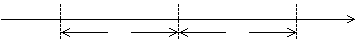
\includegraphics[scale=1.3]
{src/images/lbk-graphics/str6c.pdf}} ;
\node at (-2.6,.5){\small  $0$} ;
\node at (0,.5){\small  $1$} ;
\node at (0,-.75) {\small  $N$} ;
\node at (1.28,-.25){\small  $TL$} ;
\node at (-1.28,-.25) {\small  $SL$} ;
\node at (2.6,.5){\small  $k$} ;
\node at (4,0) [right]{\small  $x$} ;
\end{tikzpicture}
\end{center}
\vse\caption{\small Domains on the $x$-axis in 
which $\EuScript{B}$ is timelike (TL), 
null (N), and spacelike (SL)}\label{fig7.1}
\end{figure}

thus proving lemma~7.4.
% \newpage
\hbf{Linearly independent orthogonal tetrads in 
$\mbb{M}$} Now we examine the nature of the 4-vectors 
in a linearly independent orthogonal tetrad 
$\{\EuScript{B}_{(\gkm)}\}$  in $\mbb{M}$. Let
\begin{align}\label{geom.7} 
h_{\gkm\nu}\equiv\{\EuScript{B}_{(\gkm)}\dotp 
\EuScript{B}_{(\nu)}\}=\tilde{\EuScript{B}}_{(\gkm)}
\gky\,\EuScript{B}_{(\gkm)}, \quad 
\gkm ,\; \gkn=0,\;1,\;2,\;3,
\end{align} 
be the sixteen Minkowski dot-products of the 4-vectors 
of this tetrad. Since  $\{\EuScript{B}_{(\gkm)}\}$  is 
assumed to be orthogonal, we have
\begin{align}\label{geom.8} 
h_{\gkm\nu}=0,\quad \gkm \neq \gkn.
\end{align} 
Also, since $\{\EuScript{B}_{(\gkm)}\}$ is assumed to 
be a linearly independent  tetrad, it obviously 
provides a \textsl{basis} for $\mathbb{M}$ and we may 
expand an \textbf{arbitrary} 4-vector 
$\EuScript{A}\in\mathbb{M}$ in this basis as
\begin{align}\label{geom.9}
\EuScript{A} = 
\sum_{\gkm=0}^{3}\gkl_\gkm\EuScript{B}_{(\gkm)},
\end{align}
where $\gkl_\gkm$ are four scalars. 
% Then, we have (see \eqref{} 
% \begin{align}\label{geom.9}
% \EuScript{A}\dotp\EuScript{A}=\EuScript{A}^2
% &=\sum_{\gkm=0}^{3}\gkl_\gkm
% \EuScript{B}_{(\gkm)}\dotp 
% \sum_{\gkr=0}^{3}\gkl_\gkr{\EuScript{B}_{(\gkr)
% }}
% \notag\\ &=\gkl_0^2 h_{00}+\gkl_1^2
% h_{11}+\gkl_2^2 h_{22}+\gkl_3^2 h_{33}.
% \end{align}
Now, let us assume that one of the members of the 
tetrad $\{\EuScript{B}_{\gkr} \}$,  say, 
$\EuScript{B}_{(3)}$, is \textsl{null}. Then, from
Eqns.~\break\eqref{geom.8} and \eqref{geom.9}, we note that
\begin{align*}
 \EuScript{A}\dotp \EuScript{B}_{(3)}=0.
\end{align*}
This requires that  $\EuScript{B}_{(3)} $ is orthogonal 
to every 4-vector
$\EuScript{A}\in \mbb{M}$ as  $\EuScript{A}$ is a 
perfectly arbitrary 4-vector of $\mbb{M}$. But that is 
impossible and the lemma 7.8 follows: Thus, it follows 
that 
\Lem No member of a linearly independent, orthogonal 
tetrad of 4-vectors in $\mbb{M}$ can be a null vector.

These lemmas 7.1, 7.2, 7.3 and 7.4 together  rule out 
the possibility that a linearly independent,   
orthogonal tetrad of 4-vectors has a null-vector 
member, or, has more than one timelike member. This,  
in turn, implies that a linearly independent orthogonal 
tetrad $\{\EuScript{B}_{(\gkm)}\}$ in $\mbb{M}$ must be 
of one one of the following two types:
\begin{description}
\item[4s-tetrad:~] A tetrad 
$\{\EuScript{B}_{(\gkm)}\}$ with four 
spacelike 4-vectors. 
\item[1t3s-tetrad:~] A tetrad 
$\{\EuScript{B}_{(\gkm)}\}$ 
which has one timelike and three spacelike 4-vectors.
\end{description}
Now, we shall show that only a \textbf{4s-tetrad} does 
not exist in $\mathbb{M}$. For that 
purpose, we consider an \textbf{arbitrary} 4-vector 
$\EuScript{A}$ and its squared-Minkowski-norm
\begin{align}\label{geom.10}
\EuScript{A}^2 =h_{00}(a_0)^2+ h_{11}(a_1)^2
+ h_{22}(a_2)^2+ h_{33}(a_3)^2.
\end{align}
Suppose the tetrad $\{\EuScript{B}_{(\gkm)}\}$ is of 
the type $4s$. Then, evidently  $\EuScript{B}_{(0)}^2 = 
h_{00}$, $\EuScript{B}_{(1)}^2=h_{11}$, 
$\EuScript{B}_{(2)}^2 =h_{22}$,  
$\EuScript{B}_{(3)}^2=h_{33}$  are all positive. This 
implies  $\EuScript{A}^2>0$ for an arbitrary 4-vector 
$\EuScript{A}$ which is certainly \textsl{not} true. 
Hence a  linearly independent orthogonal tetrad of the 
$4s$-type does not exist in $\mathbb{M}$.

Finally, we consider a linearly independent orthogonal 
tetrad $\{\EuScript{B}_{(\gkm)}\}$ of the type 
$\mathbf{1t3s}$. Let us name the  timelike member of 
this tetrad as $\EuScript{B}_{(0)}$, and the remaining  
three spacelike members as $\EuScript {B}_{(1)}, 
\EuScript {B}_{(2)}, \EuScript {B}_{(3)}$. 
% For such 
% tetrad, we note that $h_{00}$ is positive, 
% $h_{11},h_{22},h_{33}$ are all negative and  
% $h_{\gkm\gkn}=0,\;\gkm\neq\gkn$. 
Then, the sixteen scalar products associated with this 
tetrad are given by
\begin{align*}
\hspace*{-3mm}h_{\gkm\gkn}\equiv \EuScript{B}_ {
(\gkm)}\dotp\EuScript{B}_ { (\gkn)} 
=\begin{paray}{cccc}
h_{00}&h_{01}&h_{02}&h_{03}\\
h_{10}&h_{11}&h_{12}&h_{13}\\                          
h_{20}&h_{21}&h_{22}&h_{23}\\
h_{30}&h_{31}&h_{32}&h_{33}
\end{paray}\,.
\end{align*}
We may expand an arbitrary 4-vector $\EuScript{A}$ in 
the basis provided by $\{\EuScript{B}_{(\gkm)}\}$ as
\begin{align*}
&\EuScript{A}=\sum_{\gkm=0}^3
\gkl_{(\gkm)}\EuScript{B}_ { (\gkm)},\text{ where }
 \gkl_{(\gka)}\equiv\EuScript{A}\dotp \EuScript 
{B}_{(\gka)}.
\end{align*}
We also note that
\begin{align*}
&\EuScript{A}^2 \equiv \EuScript{A}\dotp\EuScript{A}= 
h_{00}(a^0)^2\nt-\nt|h_{11}|(a^1)^2\nt-\nt 
|h_{22}|(a^2)^2\nt -\nt|h_{33}|(a^3)^2.
\end{align*}
Clearly, the scalar $\EuScript{A}^2$ above can assume 
all values  $\gtreqqless 0$, depending on the 4-vector 
$\EuScript{A}$. These expansion formulae cover all 
vectors of $\mathbb{M}$ they evidently show that  
orthogonal bases (\ie linearly independent orthogonal 
tetrads) of the \textbf{type 1t-3s} certainly exist in 
$\mathbb{M}$. This observation, together with the 
previously made observations that any other type of 
linearly independent orthogonal tetrads  do not exist 
in $\mathbb{M}$, lead to the following important lemma:

\Lem Every  \textsl{linearly independent orthogonal 
tetrad} of 4-vectors in $\mbb{M}$ must necessarily 
consist of one timelike vector and three spacelike 
vectors.

\subsection{Constructing an orthonormal 
tetrad}\index{orthonormal tetrad ! construction}  
\dfnb A set of four mutually orthogonal 4-vectors, 
say,\break $\{\dnot,\dwon,\dtwo, \dtri\}$ in which $\dnot$ is 
a timelike unit-4-vector while $ \dwon, \dtwo, \dtri $ 
are spacelike,  unit-4-vectors, is called an 
\textsl{orthonormal  tetrad}. 

The $16$ real numbers (vector components) in an 
orthonormal tetrad  have to satisfy  $4$ conditions 
of normality and ${}^4 C_2  =6$ conditions of 
orthogonality. Therefore, \textit{an orthonormal 
tetrad is specified by $16-4-6 = 6$ independent real 
parameters.}

Often, there arises a need to find an orthonormal 
tetrad in which one of its members, which can either be 
a timelike unit vector or, a spacelike unit vector, is 
specified. This requires determining $12$ unknowns 
satisfying $9$ conditions ($3$ conditions of 
normality and ${}^4 C_2 =6$ conditions of 
orthogonality). Such a system of under-determined 
equations is certainly solvable and possesses multiple 
solutions. To obtain any one such solution, we 
may choose any $3$ unknowns out of the $12$ in an 
arbitrarily manner (say, set equal to zero). Then, we 
obtain a deterministic system of $ 9 $ equations in 
$9$ unknowns  solving which we obtain the desired 
orthonormal tetrad.

\exmnp  {Construct an orthonormal tetrad which has\lbk
$T^\gkm=(2,1,0,0)$ as its timelike member.} 

\soln $\EuScript{U}_\gkm=(a,b,0,0)$ would be orthogonal 
to $T^\gkm$ if we set\lbk $2a+b=0$ which gives 
$b=-2a$. Thus, $\EuScript{U}_\gkm=(a,-2a,0,0)$. Then, 
an inspection tells us that  $\EuScript{V}_\gkm 
=(0,0,c,0)$ and $ W_\gkm =(0,0,0,d)$ are mutually 
orthogonal and orthogonal to $T^\gkm$ and 
$\EuScript{U}_\gkm$. On normalising these four vectors, 
we get the required orthonormal tetrad:
\begin{align*}
\dnot^\gkm & =(2,1,0,0)/\sqrt{3}, \quad\dwon^\gkm 
=(1,-2,0,0)/\sqrt{3}, \\
 \dtwo^\gkm&=(0,0,1,0) ,\qquad 
\quad\dtri^\gkm=(0,0,0,1).  
\end{align*}\ebxup

\subsection{Lorentz frames}
In a Lorentz frame  $S$ suppose we are given an 
orthonormal tetrad $\{\dnot, \dwon, \dtwo,\dtri\}$ with 
$\dnot$ as its timelike member. Then, if the  zeroth 
contra component of $\dnot$ is negative,  we multiply 
the vector $\dnot$  by $-1$ and make its zeroth contra 
component positive\footnote{Of course, one can work 
with  covariant components as well.}. This makes 
$\dnot$ \textsl{future-pointing}. Next, if necessary, 
we re-order the spacelike-triplet of unit vectors 
$\dwon, \dtwo,\dtri$ such that 
\begin{align*}
\det\begin{vmatrix}
 \dnot^0&\dnot^1&\dnot^2&\dnot^3\\
 \dwon^0&\dwon^1&\dwon^2&\dwon^3\\
 \dtwo^0&\dtwo^1&\dtwo^2&\dtwo^3\\
 \dtri^0&\dtri^1&\dtri^2&\dtri^3\\
\end{vmatrix}=+1.
\end{align*}
Then, we say that the new orthonormal tetrad so 
obtained is \textsl{positively oriented}. This way,  if 
necessary, by changing the sign of its timelike  unit 
vector, and, again, if necessary,  re-ordering its 
spacelike-triplet of unit vectors, we may obtain a 
\textsl{future-pointing,  positively-oriented, 
orthonormal tetrad} from any  arbitrary orthonormal 
tetrad. In what follows, unless otherwise stated, all 
orthonormal tetrads that we consider are to be assumed 
as future-pointing and  positively-oriented. 
\index{orthonormal tetrad ! future-pointing, 
positively-oriented}
\dfnargb{Lorentz frame} A future-pointing, positively 
oriented, orthonormal tetrad of 4-vectors shall be 
called a Lorentz frame.

\subsection{Changing from one Lorentz frame to 
another}
To discuss the \textsl{change of basis} in 
$\mathbb{M}$, we use the  notation of row and column 
\textsl{stacks} of 4-vectors
\begin{align*}
\tilde{\mathbb{B}}\equiv(\EuScript{X}\,
\EuScript{Y}\, \EuScript{Z}\, \EuScript{W}) ,\quad
\mathbb{B}\equiv
\bpa{l}
\EuScript{X}\\ \EuScript{Y}\\ \EuScript{Z}\\ 
\EuScript{W}
\epa .
\end{align*}
Here, we may remind the reader that these two objects 
$\mathbb{B}$ and $\tilde{\mathbb{B}}$  are \textsl{not} 
vectors and we have introduced this notation to 
facilitate the use of the matrix method in our 
calculations. Using this notation, we may 
conveniently refer to a basis of 
$\mathbb{M}$ by its row-stack 
and call it the $\tilde{\mathbb{B}}$-basis, 
$\tilde{\mathbb{B}}'$-basis and so on.

We may also note that a Lorentz matrix (Cf. 
Eqn.\eqref{geom.1}) may now be expressed as 
\begin{align*}\tag{7.1a}
 L =\tilde{\mathbb{B}}\equiv 
(\EuScript{X} \EuScript{Y} \EuScript{Z} \EuScript{W}).
\end{align*}
Therefore,
\begin{align*}\tag{7.1b}
\det{L}= \det{\tilde{\mathbb{B}}}\equiv 
\det{(\EuScript{X}\, 
\EuScript{Y}\, \EuScript{Z}\, \EuScript{W})},\quad 
?L^0_0? 
=\EuScript{X}^0>0.
\end{align*}
When the orthonormal tetrad $\{\EuScript{X}\,  
\EuScript{Y}\,  \EuScript{Z} \, \EuScript{W}\}$ is 
future pointing and  positively oriented (\ie a 
Lorentz 
basis),  we have $\det{\tilde{\mathbb{B}}}=+1$ and 
$\EuScript{X}^0>0$ so that the  Lorentz matrix $L$ in 
Eqn.(7.1a) is proper and orthochronous.

Let $\tilde{\mathbb{B}}\equiv (\EuScript{X}\, 
\EuScript{Y}\, \EuScript{Z}\,  \EuScript{W})$ be a 
Lorentz basis of $\mathbb{M}$ and $T$  be a proper 
orthochronous Lorentz matrix. Then,
 \begin{align}\label{geom.11}
&\bpa{l} 
\EuScript{X}'\\\EuScript{Y}'\\\EuScript{Z}'\\
\EuScript{W}'\epa 
=\bpa{cccc}
T^1_{\,.1}& T^1_{\,.2}&T^1_{\,.3} & T^1_{\,.4}\\
T^2_{\,.1}& T^2_{\,.2}&T^2_{\,.3} & T^2_{\,.4}\\
T^3_{\,.1}& T^3_{\,.2}&T^3_{\,.3} & T^3_{\,.4}\\
T^4_{\,.1}& T^4_{\,.2}&T^3_{\,.3} & T^4_{\,.4}
\epa 
\bpa{l}
\EuScript{X}\\\EuScript{Y}\\\EuScript{Z}\\\EuScript{W}
\epa 
\end{align}
which may be written compactly as
\begin{align}\label{geom.12}
\mathbb{B}'= T \mathbb{B},
\end{align}
is also a basis of $ \mathbb{M}$ because the matrix $T$ 
is non-singular. Taking the transpose of this matrix 
equation, we obtain
\begin{align}\label{geom.13}
\tilde{\mathbb{B}}'= \tilde{\mathbb{B}}\tilde{T}.
\end{align}
Since the original basis is a Lorentz basis, the matrix 
$\tilde{\mathbb{B}}$ is clearly  proper and 
orthochronous. Also, we have taken $T$ to be a proper, 
orthochronous Lorentz matrix. Now,  by the 
\textsl{group-nature} of pro-\break per, orthochronous, Lorentz 
matrices, it follows that  the product (Lorentz) matrix 
$\tilde{\mathbb{B}}'= \tilde{\mathbb{B}}\tilde{T}$ is 
also proper and orthochronous. In other words, the new 
basis $\mathbb{B}'$ is positively oriented and 
future-pointing and hence is a Lorentz basis. Thus,  we 
arrive at the following lemma:

\Lem If $\mathbb{B}$ is a Lorentz basis for 
$\mathbb{M}$ and $T$ is any orthochro-\break nous proper 
Lorentz matrix, then the $\mathbb{B}'= T \mathbb{B}$ is 
also a Lorentz basis.

This lemma clearly points out at the possibility of  
generating an infinite number of Lorentz bases in 
$\mathbb{M}$,  obtainable from one another, through 
appropriate choices of the {orthochronous, proper, 
Lorentz matrix} $T$.

\subsection{Canonical forms of 4-vectors}
\index{4-vector ! canonical forms of} \index{Lorentz 
frame}
Every 4-vector assumes its canonical form in an  
appropriate  Loren\break tz frame, i.e., when referred to a 
suitable future-pointing, positive\break ly-oriented, 
orthonormal  tetrad. Below, we discuss the canonical 
forms of  timelike, null  and  spacelike 4-vectors. 
First, we note the following convenient canonical form 
of an arbitrary 4-vector:

\Lem Every 4-vector $\EuScript{A}:~A^\gkm =(a^0, 
\veca{a})$ may be brought to the {general canonical 
form} 
\begin{align}\label{geom.14} 
A^\gkm =(a^0, a ,0,0), \quad a\equiv |\veca{a}|, 
\end{align} 
by an orthochronous proper Lorentz transformation of 
the form\footnote{The notation $A\oplus B$ stands for 
the \textsl{direct-sum} of the square matrices $A$ and 
$B$. If $A$ and $B$ are square matrices of dimensions 
$n$ and $ m $, then $A\oplus B$ is the block-matrix  of 
dimension $n+m$ given by
\begin{align*}
 A\oplus B = \bpa{cc}   A&O_{nm}\\O_{mn}&B
\epa    ,
\end{align*}
where $O_{nm}$ is a zero matrix with $n$ rows and  $m$ 
columns and $O_{mn}$ is a zero matrix with $ m $ rows 
and and $n$ respectively.} $L=1\oplus R_3$ where  $R_3$ 
is a suitable 3-rotation. \prf  Define the unit 
3-vector  $ \uvec{\ell} = \veca{a}/a $  and determine 
two other unit 3-vectors $ \uvec{m}  $ and $\uvec{n}$ 
such that  $\{ \uvec{l}, \uvec{m},\uvec{n}\}$  is a 
right-handed orthonormal triad of 3-vectors. Construct 
the $3\times3$ proper orthogonal matrix
\begin{align*}
 R_3=\bpa{ccc}
l_x&l_y&l_z\\m_x&m_y&m_z\\n_x&n_y&n_z\epa 
\end{align*}
and the  orthochronous proper Lorentz matrix
\begin{align*}
L=1\oplus R_3=\bpa{cccc}   1&0&0&0\\0&l_x&l_y&l_z\\
0&m_x&m_y&m_z\\0&n_x&n_y&n_z\epa    .
\end{align*}
Then, we have\\
 \begin{align*}
\EuScript{A'}=L\EuScript{A} =\bpa{cccc}
1&0&0&0\\0&l_x&l_y&l_z\\
0&m_x&m_y&m_z\\0&n_x&n_y&n_z\epa 
\bpa{l}
a^0\\a_x\\a_y\\a_z\epa    =\bpa{l}
a^0\\a\\0\\0\epa    ,
\end{align*}
which is  the required canonical form  of an arbitrary 
4-vector.

\lemarg{The canonical form of a timelike 4-vector}  
If $\EuScript{A} =(a^0,\veca{a})$ is any timelike 
4-vector specified in the Lorentz frame $S$, we can 
always find an orthochronous proper Lorentz matrix $T$ 
such that
\begin{align}\label{geom.15}
\EuScript{A}' \equiv T\EuScript{A}=
\bpa{l}\gks(a^0) A\\0\\0\\0 \epa ,
\end{align}
where $A \equiv +\sqrt{\EuScript{A} 
\,\,\dotp\,\EuScript{A}}>0 $ and $ \gks(a^0)$ is the 
sign of $a^0$. \prf  Note that the given 
$\EuScript{A}$ 
has $a^0>0$ or,  $a^0>0$ depending on whether it is 
future-, or, past- pointing. Now, construct the 
{timelike unit vector} $\EuScript{K} \equiv 
\EuScript{A}/A$ with the contra-components  $k^\gkm = 
a^\gkm/A$ in the $S$-frame. Since $A > 0 $, $ k^0$ has 
the same sign as  $a^0$. Then, $\dnot$, defined by the 
contra components $\dnot^\gkm \equiv \gks(k^0) 
k^\gkm/A$ where $\gks(a^0)$ is the sign of $a^0$, is a {future-pointing, unit, timelike 4-vector}. Next,  
construct a future-pointing, positively oriented  
orthonormal tet\break rad $\{\dnot\, \dwon\, \dtwo\,\dtri\}$  
with  $\dnot$ as its timelike member. Then $L\equiv 
(\dnot\, \dwon\, \dtwo\,\dtri) $ is a   orthochronous 
proper Lorentz matrix. Therefore, $T\equiv 
\tilde{L}\gky$ is also a  orthochronous proper Lorentz 
matrix. Then
\begin{align*}
\EuScript{A}'=T \EuScript{A}=\tilde{L}
\gky\EuScript {A}  =\bpa{l}
\tdnot\gky \EuScript{A} \\
\tdwon\gky\EuScript{A}\\
\tdtwo\gky\EuScript{A}\\\tdtri
\gky\EuScript{A}] \epa =
\bpa{c}\gks(a^0) A\\0\\0\\0
\epa .
\end{align*}
Hence the lemma.

\lemarg{The canonical form of a null 4-vector} 
If $\EuScript{A} =(a^0,\veca{a})$ is any null 
4-vector, 
then there exists a Lorentz frame in which 
$\EuScript{A}$ has the components\\ 
$A^{\gkm'} =a\big(\gks(a^0),-1,0,0\big)$ 
where $a\equiv |\veca{a}|$.\\
\prf  Using the  Lemma 7.7, we can find an   
orthochronous proper Lorentz transformation $ 
?L^{\gkm'}_\nu?$ such that $A^{\gkm'}= ?L^{\gkm'}_\nu? 
?A^\nu? =(a^0,a,0,0) $. Now, since $A^{\gkm'}$ is 
null, 
and the null character of a 4-vector is invariant 
under 
a Lorentz transformation, it follows that $ a^0 = 
\gks(a^0)a $. Hence the lemma.
\lemarg{The canonical form of a spacelike 4-vector}  
If $\EuScript{A} =(a^0,\veca{a})$ is any spacelike 
4-vector, then there exists a Lorentz frame in which 
$\EuScript{A}$ has the components  $A^{\gkm'} 
=(0,A,0,0) $ where  $A \equiv +\sqrt{- \EuScript{A} 
\dotp\EuScript{A}}$. \prf  With the spacelike unit 
vector $\dwon \equiv \EuScript{A}/A$ as its second 
member, let us construct a positive orthonormal tetrad 
$\{\dnot, \,\dwon$  $\dtwo, \,\dtri\} $ and the and the 
associated orthochronous proper Lorentz transformation 
$L\equiv (\dnot \,\dwon\,\dtwo \,\break \dtri)$. Then, it is 
easy to see that  $A^{\gkm'} =?L^{\gkm'}_\nu? ?A^\nu? 
=(0,A,0,0)$. Hence the lemma.

\section{Minkowski coordinates}
In the Minkowski spacetime $\mathbb{M}$, one often 
works with a slightly different coordinate system 
$\{x_1,x_2,x_3,x_4\}$ called the Minkowski coordinate 
system which is related to the familiar 
pseudo-Carte\break sian coordinates $\{ct,x,y,z\}$ in a  
simple manner through $x_1=x,\;x_2=y,\;x_3=z,\; 
x_4=ict$.

In Minkowski coordinates, every event of $\mathbb{M}$ 
is  labelled by a unique ordered quadruplet of  
coordinates $ (x,y,z,w) $ where we use the notation $ 
w 
\equiv ict $ for convenience. If $ (x_1,y_1,z_1,w_1) $ 
and $ (x_2,y_2,z_2,w_2) $ are the coordinates of two 
events in $ \mathbb{M}$, then we define
\begin{align}\label{geom.16}
s_{12}^2&=(x_2-x_1)^2+(y_2-y_1)^2+(z_2-z_1)^2+(w_2 
-w_1)^2\notag\\& 
=(x_2-x_1)^2+(y_2-y_1)^2+(z_2-z_1)^2-c^2(t_2-t_1)^2.
\end{align}
as the invariant squared-interval between the two 
events.

However, we may recall that, in real coordinates  
$\{ct,x,y,z\}$, we define
\begin{align}\label{geom.17}
s_{12}^2&=c^2(t_2 -t_1)^2 -(x_2-x_1)^2 -(y_2-y_1)^2 
-(z_2-z_1)^2
\end{align}
as the invariant squared-interval between the same two 
events\lbk $(ct_2,x_2,y_2,z_2)$ and 
$(ct_1,x_1,y_1,z_1)$. In special relativity, both 
the\lbk choices, namely, \eqref{geom.16} and 
\eqref{geom.17} are used for the invariant  
squa\break red-interval. However, one must consistently 
use\footnote{Such a change of signatures can be a 
non-trivial procedure, especially in general 
relativity: See for example, J.L.Synge, Relativity: 
The 
General Theory, North Holland Publishing Company, 
Amsterdam, 1971, Appendix A.} either  
Eqn.\break \eqref{geom.16}, or,  Eqn.\eqref{geom.17}.

To distinguish between the choices \eqref{geom.14} and 
\eqref{geom.15}, one uses the {signature}  of the 
quadratic forms  \eqref{geom.16} and \eqref{geom.17}. 
The signature  of the invariant squared-interval is 
defined as ``the number of positive terms in the 
invariant squared-interval {minus} the number of 
negative terms'' in it. Thus, the squared-interval in 
\eqref{geom.16} has the signature $+2$ whereas that in 
\eqref{geom.17} has thesignature $-2$.

It is important to note that only in this chapter~7,  
we  use the imaginary coordinate $ x_4=ict $ and an 
invariant squared-interval with signature +2. However, 
in the rest of this book, we work with the real 
time-coordinate $ x^0 \equiv ct $ and an invariant, 
squared-interval in the signature -2 convention.

\subsection{Some notes on working with Minkowski\\
coordinates}
\begin{enumerate}
\item In Minkowski coordinates, a general event of 
spacetime is marked by the coordinate quadruplet
 \begin{align*}
(x_1,x_2,x_3,x_4)\equiv (x,y,z,ict)\equiv 
(\veca{r},ict).
\end{align*}\\
The 4-position vector $\EuScript{X}$ of an event would
therefore be represented by the $4$-dimensional column 
vector
\begin{align}\label{geom.16}
\EuScript{X}\mapsto X=\bpa{l}  x_1\\x_2\\x_3\\x_4
\epa =\bpa{l}  x\\y\\z\\ict \epa .
\end{align}

\item A transformation from one Lorentz frame $S$ to 
another, say $ S' $, corresponds to  the coordinate 
change
\begin{align}\label{geom.16}
x'_{\gkm}= L_{\gkm\nu}x_{\nu},
\end{align}
from one Minkowski coordinate change system  
$\{x_\gkm\}$ to another $\{x'_\gkm\}$, where 
$\;\gkm=1,2,3,4\}$. Here,  as usual, we have adopted 
the {summation convention} of summing over 
\textsl{repeated indices}. In matrix notation, the  
Lorentz transformation \eqref{geom.16} may be 
expressed 
as
\begin{align}\label{geom.21x}
 \bpa{l}x'_1\\x'_2\\x'_3\\x'_4 \epa 
=\bpa{cccc}
L_{11} & L_{12} &L_{13} &L_{14}\\
L_{21} & L_{22} &L_{23} &L_{24}\\
L_{31} & L_{32} &L_{33} &L_{34}\\
L_{41} & L_{42} &L_{43} &L_{44}\\ \epa 
\bpa{l} x_1\\x_2\\x_3\\x_4 \epa .
\end{align}
We may also write Eqn.\eqref{geom.21x}  compactly as
\begin{align}\label{geom.22x}
X'=LX.
\end{align}
in an obvious notation. 

\item In every Minkowski coordinate system, the first  
three coordinates of an event must be real and the 
fourth must be pure imaginary. This clearly requires 
that the Lorentz matrix $L$ in Eqn.\eqref{geom.21x} 
must have the \textsl{reality structure}
\begin{align} \label{geom.23x}
 L=\bpa{cccc}
 r & r &r &i \\
 r & r &r &i \\
 r & r &r &i \\
 i & i &i &r
\epa ,
\end{align}
where $r$ and $i$ stand for ``real'' and ``imaginary''
respectively.

\item Recall that the special  theory of relativity 
requires that the real number
\begin{align} \label{geom.21}
&(\tilde{X}_2-\tilde{X}
_1)(X_2-X_1)\notag\\&=(x_2-x_1)^2+ 
(y_2-y_1)^2+ (z_2-z_1)^2-c^2(t_2-t_1)^2,
\end{align}
associated with every pair of events $X_1$ and $X_2$ 
is 
a Lorentz scalar. Thus, we must have,
\begin{align} \label{geom.22}
&(\tilde{X}'_2-\tilde{X}'_1)
(\tilde{X}'_2-\tilde{X}'_1)=
(\tilde{X}_2-\tilde{X}_1)(\tilde{L}
L)(X_2-X_1) \notag \\&=
(\tilde{X}_2-\tilde{X}_1)(X_2-X_1).
\end{align}
{As the matrix $ \tilde{L}L $ is symmetric, and $ 
(X_2-X_1) $ is arbitrary}, this requires
\begin{align}\label{geom.26x}
 \tilde{L}L =E,\quad (L^{-1}  = \tilde{L}),
\end{align}
where $E$ is the $ 4\times4 $ unit matrix. Thus, $L$  
is a (complex) orthogonal matrix with the special 
reality  structure given in Eqn.\eqref{geom.23x}. 
Equation \eqref{geom.23x}  is also called the 
\textsl{Lorentz condition} and, when satisfied,  it 
guarantees that a (complex) $ 4\times 4 $ matrix $L$ 
which has the reality-structure given in 
Eqn.\eqref{geom.23x}, is a Lorentz transformation 
matrix in Minkowski coordinates. 
\item The invariant scalar product $\EuScript{A}\dotp 
\EuScript{B}$ of two 4-vectors is given by
\begin{align}\label{geom.24}
\EuScript{A}\dotp \EuScript{B} = \tilde{A}B
= \tilde{A}E B,
\end{align}
which clearly shows that the unit matrix $E$ is the 
\textsl{metric-matrix} in Minkowski coordinates.

\item Because the metric matrix is $E$, the 
(corresponding) associate components of an arbitrary 
tensor would all be equal in Minkowski coordinates. 
For 
example, $?{T}^\gka_{\gkm\nu}?  = ?{T}_{\rho\gkm\nu} ? 
= ?{T}^\rho_\gkm^\nu ?$ etc. However, one must note 
that the associate components of a tensor, although 
equal in Minkowski coordinates, would not be equal, in 
general, in some other coordinate system (such as the 
real coordinates  $ ct,x,y,z$). \item The equality of 
the corresponding associate components of a tensor in 
Minkowski coordinates, permits one to drop the the 
notational distinction between contra- and co-indices 
and write all tensor indices, say,  as suffixes. This 
is a great notational simplification and is one of the 
advantages of using $ x_4=ict $. However, as already 
remarked,  care must be exercised while transforming 
back to real coordinates $ ct,x,y,z $ and the 
appropriate tensorial transformation rule be used to 
get the right tensor components in real coordinates.

\item In particular, we may represent a 4-vector 
$\EuScript{A}$ in   Minkowski coordinates  by the 
column vector 
\begin{align}\label{geom.25}
\EuScript{A}\mapsto A=\bpa{l}
a_1\\a_2\\ a_3\\  a_4 \epa .
\end{align}
where  $a_1,a_2, a_3, a_4$ are called the Minkowski 
components of $\EuScript{A}$. It is important to note 
that the indices are \textsl{all sub-scripts} now. 
\item Another important simplification achieved by 
using $ x_4=ict $ is that, when one transforms from 
one 
Minkowski system to another, the transformation law of 
an arbitrary second rank tensor $T=(?T_\gkm\nu?) $ 
becomes the {matrix similarity transformation} $ 
T'=LTL^{-1} =LT\tilde{L}$ where $L$  is the Lorentz 
transformation matrix. This is a definite advantage, 
especially in this chapter where we use matrix methods 
to  study the properties of the Lorentz transformation.

% In the literature, it is called the
% {Weyl unitary trick}\footnote{R.Gilmore, Lie Groups, 
% Lie Algebras  and Some of Their Applications, John 
% Wiley, New  York, 1974, p.41}.

\item One must have already noticed the change in the 
numbering of the coordinates: Unlike in real  
coordinates, where the numbering is from $0$ to $3$, 
the numbering in Minkowski coordinates is from from  
$1$ to $4$.
\end{enumerate}

\section{2-flats in the Minkowski world}
Let  $\EuScript{A}$, $\EuScript{B}$ and $\EuScript{C}$ 
be three {linearly independent} position  4-vectors of 
three events in $\mathbb{M}$. 

\dfnargb{General 2-flat}  A two-dimensional subspace 
of 
$ \mathbb{M}$, defined as the totality of all events $ 
X $ given by
\begin{align}\label{geom.26}
 X = \gkl\EuScript{A} +\gkm \EuScript{B}+ \EuScript{C},
\end{align}
where $\gkl,\gkm $ are any two real numbers in 
$-\infty< \gkl,\gkm< +\infty $, is called a 2-flat of 
$\mathbb{M}$.
\dfnargb{2-flat through the origin} When 
$\EuScript{C}=0$ in Eqn.\eqref{geom.26}, we say that 
the  2-flat passes through, or,  contains the origin 
of 
$\mathbb{M}$.

Such a 2-flat through the origin is completely   
determined by the basis (i.e., linearly independent)  
4-vectors $\{\EuScript{A}, \,\EuScript{B} \}$. From 
now 
on, unless otherwise stated, {a 2-flat means a 2-flat 
through the origin only}.

\Lem A basis $\{\EuScript{A}, \,\EuScript{B} \}$ of a 
2-flat can always chosen to be an orthogonal basis. 
\prf Let $\{\EuScript{A}, \,\EuScript{B}\}$ be an 
arbitrary basis of the 2-flat. We define a new pair of 
4-vectors by
\begin{align}\label{geom.27}
 \EuScript{X} =\gka\EuScript{A}+\gkb
\EuScript{B},\quad \EuScript{Y}
=\gkg \EuScript{A}+\gkd\EuScript{B},
\end{align}
where $ \gka,\gkb,\gkg,\gkd $ are any four real numbers
satisfying
\begin{align} \label{geom.28}
 \gka\gkd-\gkb\gkg\neq 0.
\end{align}
Now, if we require the new basis $\{\EuScript{X}, 
\EuScript{Y}\} $ to be an  orthogonal pair of  
4-vectors, we see that the {four} real coefficients $ 
\gka,\gkb,\gkg,\gkd $ have to satisfy the following 
{two} real conditions
\begin{align}\label{geom.29}
&\gka\gkd-\gkb\gkg\neq
0,\notag\\& \EuScript{X}\dotp \EuScript{Y}= \gka\gkg
\EuScript{A}^2+(\gka\gkd+ \gkb\gkg)
\EuScript{A} \dotp \,
\EuScript{B} +\gkb\gkd\EuScript{B}^2 =0.
\end{align}
It is not difficult to see that these conditions may be 
satisfied in several ways (See the example 7.3 below.). 
Hence the lemma.
\exm Give at least one explicit solution of 
Eqn.\eqref{geom.29} for the parameters 
$\gka,\;\gkb,\;\gkg,\;\gkd $ in all the possible 
cases, 
namely,  $\EuScript{A}$ and $\EuScript{B}$ are 
(i)~timelike-timelike,  (ii)~timelike-spacelike, 
(iii)~space\break like-spacelike  and (iv)~timelike-null  
(v)~spacelike-null.

\soln First, we note that two null vectors are never 
orthogonal so that the pair 
$\EuScript{A},\EuScript{B}$ 
must have  have at least one non-null vector. Let 
$\EuScript{A}$ be the  non-null vector. Then, we obtain 
a special solution of Eqn.\eqref{geom.29} as followx: 
First,  we satisfy the condition 
$(\gka\gkd-\gkb\gkg)\neq 0$ by setting  
$(\gka\gkd-\gkb\gkg)= 1$. In addition, we set $\gkd=1$ 
in $\gka\gkd-\gkb\gkg =1$  and obtain 
$\gka=1+\gkb\gkg$. Plugging this into  
Eqn.\eqref{geom.29}, we get
\begin{align*}
(1+\gkb\gkg) \gkg\EuScript{A}^2 +(1+2\gkb\gkg)
\EuScript{A} \dotp\EuScript{B} + \gkb\EuScript{B}^2=0.
\end{align*}
Now, if we choose $\gkb=0$, we get $\gka=1+\gkb\gkg=1$ 
and Eqn.(7.29b)  requires 
$\gkg=-\EuScript{A}\dotp\EuScript{B}/\EuScript{A}^2$. 
Thus, finally, we have
\begin{align}\label{b}
\gka=\gkd=1, \;\gkb=0,\;
\quad *{and} \gkg= -\EuScript{A}
\dotp\EuScript{B}/\EuScript{A}^2,
\end{align}
which is a special solution of Eqn.\eqref{geom.29}. As 
a check, that it has all the desirable properties 
mentioned in the statement of the  problem (7.2) 
above, 
we verify the case (i) in which $\EuScript{A}$ and 
$\EuScript{B}$ are  both timelike.  Then, we  
normalize 
both the timelike vectors $\EuScript{A}$ and 
$\EuScript{B}$. Now, Eqn.\eqref{b} gives $\gka=\gkd=1$,
$\gkb=0$, and $\gkg= -\EuScript{A} \dotp\EuScript{B}$ 
so that
\begin{align*}
 \EuScript{X}&=\gka\EuScript{A}+\gkb\EuScript{B}
=\EuScript{A}  \text{ and }
\EuScript{Y}=\gkg\EuScript{A}+\gkd\EuScript{B}\\
&=(\EuScript{A}\dotp\EuScript{B}/\EuScript{A}
^2)\EuScript{A}
+\EuScript{B}.
\end{align*}
Clearly, $\EuScript{X} \dotp\EuScript{Y}=-\EuScript{A} 
\dotp\EuScript{B}+\EuScript{A} \dotp\EuScript{B}=0$ as 
required. Similarly, one may verify that \eqref{b} is 
a 
special solution of Eqn.\eqref{geom.29} covering 
\textsl{all the remaining possible cases.}  \ebx


Now, in view of the orthogonality properties of  
4-vectors established in \S~7.2.1, it follows that a  
orthogonal basis of a 2-flat must belong to one of the 
following types:
\begin{description}
\item[\textsl{st} pair] A pair of 4-vectors in which 
one is a unit spacelike vector and the other a unit 
timelike vector. \item[\textsl{sn} pair] A pair of 
4-vectors in which one is a unit  spacelike vector  
and 
the other is a null vector.
\item[\textsl{ss} pair] A pair of 4-vectors in which 
both the vectors are unit spacelike vectors. 
\end{description}
Furthermore, we shall prove below that any given 
2-flat 
admits only one of the above types of orthogonal-bases.

Let the 2-flat under consideration be generated by the 
orthogonal basis provided by $\EuScript{A}$ and 
$\EuScript{B}$. Then, we must have 
$\EuScript{A}\dotp \EuScript{B}=0$ where 
$\EuScript{B}$ is 
not a scalar multiple of $\EuScript{A}$. Let us define 
a new orthogonal basis through the transformation 
\begin{align} \label{geom.30}
\EuScript{X}=\gky\EuScript{A}+\gkm\EuScript{
B},\quad\EuScript{Y}=\gky'\EuScript{A}
+\gkm'\EuScript{B}.
\end{align}
Then the scalars $\gky,\gkm,\gky',\gkm' $ have to 
satisfy 
the two conditions
\begin{align}  \label{geom.31}
D\equiv \gky\gkm'-\gky'\gkm\neq
0,\quad\EuScript{X}\dotp\EuScript{Y}
=\gky\gky'\EuScript{A}
^2+\gkm\gkm'\EuScript{B}^2=0,
\end{align}
which when true yield the vectors $\EuScript{X}$ and
$\EuScript{Y}$ with the  squared\lbk Minkowski-norms
\begin{align} \label{geom.32}
\EuScript{X}^2=\gky^2\EuScript{A}
^2+\gkm^2\EuScript{B}^2,\quad
\EuScript{Y}^2=\gky'^2\EuScript{A}
^2+\gkm'^2\EuScript{B}^2.
\end{align}

\hbf{Case of an \textsl{st} pair} If 
$\{\EuScript{A}, \,\EuScript{B}\}$ is a 
\textsl{st} pair, then we have $\EuScript{A}^2=1 $, 
$\EuScript{B}^2=-1$, and $\EuScript{A}\dotp 
\EuScript{B} 
=0$. These conditions together with 
Eqns.\eqref{geom.30} and
\eqref{geom.31} require that
\begin{gather} \label{geom.33}
D\equiv \gky\gkm'-\gky'\gkm\neq 0, \;\;
\gky\gky' - \gkm\gkm'= 0, \\\label{geom.34}
\EuScript{X} ^2=\gky^2-\gkm^2, \quad
\text{and} \quad  \EuScript{Y}
^2=\gky'^2-\gkm'^2.
\end{gather}
Observe that $\EuScript{X} ^2 =\gky^2-\gkm^2$ cannot 
vanish as that requires  the transformation Jacobian 
$D$ to vanish which is impossible. For the same 
reason, 
 $\EuScript{Y} ^2 ={\gky'}^2-{\gkm'}^2$ also can not 
vanish.


Suppose that the second condition in 
Eqn.\eqref{geom.33} is satisfied with  $\gkm$ and 
$\gky'$  both being non-zero. Then, we must have
\begin{align*}
\EuScript{X}^2 =\gky^2- \gkm^2 =
(\gkm^2/\gky'^2) (\gkm'^2-\gky'^2)= -
(\gkm^2/\gky'^2) \EuScript{Y}^2.
\end{align*}
So, if  $\EuScript{X}^2$ is positive $\EuScript{Y}^2$ 
is negative and vice versa. The above equation 
obviously breaks down when either $\gkm=0$ and  
$\gky'=0$, or  when $\gkm=\gky'=0$. We shall examine 
them separately:

Suppose $\gkm=0$ and  $\gky'=0$. Then, from 
Eqn.\eqref{geom.33}, we note that $\gky\neq 0$ and 
$\gkm'\neq 0$ is the only choice which gives a $D\neq 
0$. Further, with $\gkm=0, \; \gky'=0$, and $\gky\neq 
0,\;\gkm'\neq 0$, we get  $\EuScript{X}^2 ={\gky}^2>0$ 
and $\EuScript{Y}^2 =-{\gkm'}^2 < 0$.

Similarly, when $\gkm=\gky'=0$, the two conditions in 
Eqn.\eqref{geom.32} require that $\gky\neq 0$ and 
$\gkm'\neq 0$ and we are led to   $\EuScript{X}^2 
={\gky}^2 > 0$ and $\EuScript{Y}^2 =-{\gkm'}^2 < 0$. 
Summing up, we have the following lemma:

\Lem An \textsl{st} orthogonal basis is transformed  
into another st orthogonal basis by an allowed basis  
transformation (i.e., one with $D\neq 0$).

\hbf{Case of an \textsl{ns} pair}Let $\EuScript{A}$ 
and 
$\EuScript{B}$ be an \textsl{ns} pair of vectors with 
$\EuScript{A}^2=0$ and $\EuScript{B}^2=-1$. Then, 
Eqs.\eqref{geom.30} and \eqref{geom.31} require
\begin{align*}
D=\gky\gkm'-\gkm\gky'\neq 0, \;\;
\gkm\gkm'=0,
\end{align*}
which when satisfied would make
\begin{align*}
\EuScript{X}^2=-\gkm^2,\;\;
\EuScript{Y}^2=  -{\gkm'}^2.
\end{align*}
Now, the condition $\gkm\gkm'=0$ requires that at 
least 
one of $\gkm$ and $\gkm'$ must vanish. Also, $\gkm$ 
and 
$\gkm'$ cannot vanish  simultaneously as that would 
require $D=0$ which is not true.  Thus, if 
$\EuScript{X}$ is spacelike, then $ \EuScript{Y}$  is 
null and conversely. Therefore, we arrive at the 
following lemma:

\Lem Every allowed basis transformation of a pair of 
 \textsl{sn}\lbk orthogonal vectors yields another  
\textsl{sn} orthogonal  pair.

\hbf{Case of an \textsl{ss} pair} Lastly, if 
$\{\EuScript{A},\,\EuScript{B}\}$ is an \textsl{ss} 
pair,  with $\EuScript{A}^2 =\EuScript{B}^2=-1$, the 
Eqs.\eqref{geom.29}-\eqref{geom.32} require
\begin{align*}
&D=\gky\gkm'-\gky'\gkm\neq 0,\; 
\gky\gky'+\gkm\gkm'=0,\\
&\EuScript{X}^2=-\gky^2-\gkm^2,\;\EuScript{Y}^2
=-\gky'^2-\gkm'^2,
\end{align*}
so that $\EuScript{X}$ and $\EuScript{Y}$ are both 
spacelike, and we are led to the lemma

\Lem  Every allowed basis transformation of a pair of
 \textsl{ss}\lbk orthogonal vectors yields another  
\textsl{ss} orthogonal  pair.

The  lemmas 7.11, 7.12 and 7.13 clearly show that a 
given 2-flat through the origin admits only one of the 
 
three types of orthogonal basis vector pairs. 
\begin{quote} Thus, based on the unique type of 
orthogonal basis vector pair admitted by a 2-flat 
passing through the origin of $\mathbb{M}$, we may 
address it  \textsl{uniquely} as (i) an { \textsl{st} 
2-flat}, (ii) an { \textsl{sn} 2-flat},  or as (iii) 
an 
{ \textsl{ss} 2-flat}.
\end{quote}
\exm There is considerable freedom in choosing an 
orthogonal basis pair in a given 2-flat.  Exploit that 
freedom to choose a pair 
$\{\EuScript{P},\EuScript{Q}\}$ in the 3-flat in a 
special way detailed below: The spacelike unit vector 
$\EuScript{P}$ in the pair is given by
\begin{align}\label{geom.35}
\tilde{\EuScript{P}}= (\hat{p},0),\quad \text{ where } 
\hat{p} \text{ is a unit 3-vector},
\end{align}
and, the other 4-vector $\EuScript{Q}$ in the pair, 
with components $\{\veca{q},iq_4\}$, is
\begin{align}\label{geom.36} 
(i)\;\;\;  & \text{a 
timelike unit vector when } 
\{\EuScript{P},\EuScript{Q}\} \text{is an \textsl{st} 
basis}, \notag\\
(ii)\;\; &\text{a spacelike unit vector when } 
\{\EuScript{P},\EuScript{Q}\} 
\text{ is an  \textsl{ss} basis}, \notag\\
(iii)\; &\text{and a null vector satisfying }
\veca{q}^2= 1=q_4^2, \notag\\& \text{when } 
\{\EuScript{P},\EuScript{Q}\}  \text{is an  
\textsl{sn} basis}.
\end{align}

\prf To establish this result, we begin with a basis 
pair $\{\EuScript{U},\EuScript{V}\}$ in which 
$\,\EuScript{U}$ and $\EuScript{V}$, whenever 
non-null, 
have been normalised to $\pm 1$. Next, we note that 
one 
of these vectors, say $\EuScript{U}$, must necessarily 
spacelike since a null or timelike vector cannot be 
orthogonal to another null or timelike vector. Then, 
we 
prove that in the 2-flat determined by the orthogonal 
basis-pair $\{\EuScript{U},\EuScript{V}\}$, we can 
always choose another orthogonal basis-pair $\{P,Q\}$ 
of which the spacelike vector $P$ has its temporal 
component equal to zero.

\hbf{\textsl{ss} pair} First, we consider the case 
when 
$\EuScript{U},\EuScript{V}$ is an   \textsl{ss} 
orthonormal pair. Then $\EuScript{P},\EuScript{Q}$ 
defined by
\begin{align}\label{geom.126}
&\EuScript{P}= 
\EuScript{U}\cos\gkf-\EuScript{V}\sin\gkf\notag \\
&\EuScript{Q}= 
\EuScript{U}\sin\gkf+\EuScript{V}\cos\gkf,
\end{align}
may  be checked to be another  \textsl{ss} orthonormal 
pair 
 
(Exercise~7.3). Then, with $iu_4, iv_4$ and $ip_4$ 
denoting respectively  the 4-th components of 
$\EuScript{U}, \EuScript{V}$ and $P$,  we may set $p_4 
= u_4\cos\gkf +v_4\sin\gkf=0$, as desired,  and 
determine the rotation angle $\gkf$ such that 
$\tan\gkf=(u_4/v_4)$.

\hbf{\textsl{st} pair} Secondly, when  
$\{\EuScript{U},\EuScript{V}\}$ is an  \textsl{st} 
orthonormal pair of vectors, where $\EuScript{U}$ is a 
spacelike unit vector and $\EuScript{V}$ is a timelike 
unit vector, we may define a new orthogonal pair 
$EuScript{P},\break EuScript{Q}$ by
\begin{align}\label{geom.127}
&\EuScript{P}= 
\EuScript{U}\cosh\gkf-\EuScript{V}\sinh\gkf\notag\\
&\EuScript{Q}= 
-\EuScript{U}\cosh\gkf+\EuScript{V}\cosh\gkf.
\end{align}
One can check (Exercise~7.4) that the above pair 
$\EuScript{P},\EuScript{Q}$ is also an  \textsl{st} 
orthonormal pair with $\EuScript{P}$ spacelike and 
$\EuScript{Q}$ timelike. As before, it appears that 
$p_4$ may be made equal to zero by taking  
$\tanh\gkf=(u_4/v_4)$. However, as $|\tanh \gkf|\leq 
1$, the choice $\tanh\gkf=(u_4/v_4)$ would be possible 
only if $|u_4/v_4|\leq 1$ which we will now show to be 
true as follows: The orthogonality condition 
$\tilde{\EuScript{U}}\EuScript{V} =u_4v_4 +u_3v_3 
+u_2v_2 +u_1v_1 =0$ implies
\begin{align*}
u_4^2v_4^2&=(u_3v_3+u_2v_2+u_1v_1)^2\\
&\leq(u_3^2+u_2^2+u_ 1 ^ 2 ) 
(v _ 3 ^ 2+v_2^2+v_1^2)\\
& =(1+u_4^2)(-1+v_4^2)=-1-u_4^2+v_4^2
+u_4^2v_4^2,
\end{align*}
so that $v_4^2-u_4^2\geq 1$ and consequently, 
$u_4^2/v_4^2\leq 1-1/v_4^2<1$.

\hbf{\textsl{sn} pair}Finally, when 
$\EuScript{U},\EuScript{V}$ is \textsl{sn} orthogonal 
pair 
of vectors, where $\EuScript{U}$ is a spacelike and 
$\EuScript{V}$ is null, we may define a new orthogonal 
pair 
$\EuScript{P},\EuScript{Q}$ in the 
$\{\EuScript{U},\EuScript{V}$\} 2-flat by
\begin{align}\label{geom.128}
\EuScript{P}= \EuScript{U}-k\EuScript{V},\quad 
\EuScript{Q}=\EuScript{V},
\end{align}
where $k$ is an arbitjby a suitable number so that
\begin{align*}
\veca{v}^2=q_1^2+q_2^2+q_3^2= 1=q_4^2.
\end{align*}
Thus follows the result that an orthogonal pair of  
4-vectors defining a 2-flat through the origin of 
$\mathbb{M}$ may always be chosen so as to satisfy the 
equations \eqref{geom.35} and \eqref{geom.36}. \ebx

\section{Lie algebra of the proper Lorentz 
group}
From the discussion in \S 4.4, we recall that a 
homogeneous Lorentz transformation $L$ in Minkowski 
coordinates is a linear transformation on $\mathbb{M}$ 
defined by the equations  \eqref{geom.22x}, 
\eqref{geom.23x} and \eqref{geom.26x} and that the set 
$\mathfrak{L}$ of all such Lorentz matrices $L$ form 
the matrix group $\mathsf{O}(1,3)$ called the 
homogeneous Lorentz group. The group $\mathsf{O}(1,3)$ 
is also called the \textsl{full Lorentz group}. 
Furthermore, as we observed in \S 4.4,
\begin{align*}
\mathfrak{L}_{+}=\{L\in\mathfrak{L}|\det(L)=+1\}\subset
\mathfrak{L},
\end{align*}
is a subgroup of $\mathfrak{L}$ called \textsl{proper 
Lorentz group}. Now, we consider the Lie algebra 
$\mathfrak{g}$ of the proper Lorentz group 
$\mathfrak{L}_+$.
We know\footnote{See Theorem~7.2 of Appendix~7.8} that 
(cf.Theorem~7.2 of  Appendix~7.8) an element 
$L\in\mathfrak{L}_+$, which is sufficiently close to 
the identity $E$, is an exponential $L=e^{pS}$ where 
$p$ is a real parameter and $S$ is an element from the 
Lie algebra $\mathfrak{g}$ of  $\mathfrak{L}_+$. Then, 
imposing the Lorentz condition $L^{-1}=\tilde{L}$ on 
it, we obtain, for sufficiently small values of $p$,
\begin{align}\label{geom.44}
L^{-1}=\tilde{L}= e^{-p\tilde{S}}\approx E-pS
=L= e^{pS}\approx E+pS.
\end{align}
Hence, we must have
\begin{align}\label{geom.45}
\tilde{S}= -S.
\end{align}
from which we see that  the Lie algebra $\mathfrak{g}$ 
of the proper Lorentz group $\mathfrak{L}_+$ consists 
of all $4\times4$ skew-symmetric  matrices $S$ with 
the 
specific reality structure given in  
Eqn.\eqref{geom.23x}).

The skew-symmetry of $S$ and its reality-structure in 
Eqn.\eqref{geom.23x} permits representing it as 
\begin{align}\label{geom.46}
S=\bpa{cccc}
0&h_3&-h_2&ie_1\\
-h_3&0&h_1&ie_2\\
h_2&-h_1&0&ie_3\\
-ie_1&-ie_2&-ie_3&0
\epa ,
\end{align}
where  $e_1,e_2,e_3$ and $h_1,h_2,h_3$ are the six 
independent \textsl{real} variables called the 
\textsl{Lie parameters} of the Lie group 
$\mathfrak{L}_{+}$.

\dfnargb{Parameter vectors of $L$} The 3-vectors 
$\veca{e},\veca{h}$ are called the {parameter vectors} 
of $L\in \mathfrak{L}_{+}$.

In the following paragraphs, we study, in some  
detail, 
the Lie algebra element\footnote{In Physics,  a Lie 
algebra element of a proper Lorentz transformation, 
such as $S$, is, sometimes, referred to as  a 
\textsl{infinitesimal (Lorentz) transformation}. 
Strictly speaking, an infinitesimal Lorentz 
transformation, i.e., a Lorentz transformation which 
is 
infinitesimally separated from the identity (Lorentz) 
transformation $E$ in $\mathfrak{L}_{+}$, has the 
(matrix) form $L =E+\varepsilon S$ where $E$ is the 
$4\times 4$ unit matrix (=the identity element of 
$\mathfrak{L}_{+}$), $\varepsilon$ is an infinitesimal 
real parameter ($\varepsilon^2<<\varepsilon $), and  
$S$ is the Lie algebra element corresponding to $L$.} 
$S$ associated with a proper Lorentz matrix $L$. 
\index{proper Lorentz transformation ! Lie algebra 
element of a}

It may be observed that the matrix $S$ has the 
structure of the electromagnetic field 
tensor\footnote{However, observe that the change in 
notation: The vectors $\veca{E}, \veca{B}$ of the 
electromagnetic field tensor are denoted, 
respectively, 
by $\veca{e}, \veca{h}$ in $S$.}. Exploiting this 
structural  (algebraic) similarity and using the well 
known Lorentz invariant classification of the 
electromagnetic  field (tensor) at an event of 
spacetime\footnote{See  the discussion of the 
electromagnetic field in the next chapter~8.}, we 
arrive at a useful (Lorentz invariant) classification 
(see \S~7.5.1) of the the Lie algebra elements $S$. 
This, in turn, yields a classification of the proper 
Lorentz transformations.

% \subsection{Classification of proper Lorentz
% transformations}

\index{proper Lorentz transformation ! classification 
of} 
Note that the identity transformation $E$ corresponds 
to the Lie algebra element is the zero matrix $S=0$ 
which has the parameters $\veca{e}=\veca{h}=0$. We may 
call a Lorentz transformation $L$ \textsl{non-trivial} 
if it's Lie algebra element is a non-zero matrix which 
happens when  at least one of its parameter vectors 
$\veca{e}$ and $\veca{h}$ is non-zero.

\subsection{Eigenvalues of a Lorentz matrix} 
\index{Lorentz transformation ! eigenvalues of}
In a given Lorentz basis,  (in Minkowski coordinates), 
we set up the characteristic equation for $S$ using  
Eqn.\eqref{geom.46}:
\begin{align}\label{geom.47}
 \det(S-\gkl E)=\gkl^4+(\veca{h}^2-\veca{e}^2)\gkl^2
-(\veca{h}\dotp \veca{e})^2=0.
\end{align}
The two roots of this quadratic equation in $\gkl^2$ 
are
\begin{align}\label{geom.48}
\gkl_1^2&=-(\veca{h}{\:^2}-\veca{e}{ \:^2})/2
+\sqrt{(\veca{h}{\:^2}-\veca{e}{\:^2})^2/4
+(\veca{h}\dotp\veca{e}){\:^2}},\\\notag\\ 
\label{geom.49}
\gkl_2^2&=-(\veca{h}{\:^2}-\veca{e}{\:^2})/2-\sqrt{
(\veca{h}{\:^2}
-\veca{e}{\:^2} )^2/4+(\veca{h}\dotp\veca{e}){\:^2}}.
\end{align}
Evidently $\gkl_2^2\leq 0$ and we  denote it by 
$\gkl_2^2=-\gkq_r^2$  where $\gkq_r$ is real. Then, we 
may express two of the eigenvalues in 
Eqn.\eqref{geom.49}) as $\pm i\gkq_r$, where
\begin{align}\label{geom.50}
\gkq_r^2&=(\veca{h}{\:^2}-\veca{e}{\:^2}
)/2\notag\\&\qquad
+\sqrt{ (\veca{h}{\:^2} -\veca{e}{\:^2})^2/4
+(\veca{h}\dotp\veca{e}){\:^2}}.
\end{align}
Similarly, we note that $\gkl_1^2\geq 0$ so that we 
denote it by $\gkl_1^2=\gkq_b^2 $ where  $\gkq_b^2\geq 
0$. Thus, we  may express the other two eigenvalues of 
$S$ in Eqn.\eqref{geom.48} as 
$\pm \gkq_b$, where
\begin{align}\label{geom.51}
\gkq_b^2&=-(\veca{h}{\:^2}-\veca{e}{\:^2})/2
+\sqrt{(\veca{h}{\:^2} -\veca{e}{\:^2})^2/4
+(\veca{h}\dotp\veca{e}){\:^2}}.
\end{align}
Because $L=e^{S}$, it now follows that the four 
eigenvalues of $L$ are (See Example~7.5)
\begin{align}\label{geom.52}
\gkl=e^{\pm i\gkq_r}, \quad  e^{\pm \gkq_b}.
\end{align}

Also, from the quadratic equation Eqn.\eqref{geom.47} 
in $\gkl^2$ we  identify the following two {two 
independent similarity invariants} of the Lie algebra 
element $S$:
\begin{align}\label{geom.53}
\EuScript{I}_1\equiv(\veca{h}{\:^2}-\veca{e}{\:^2}), 
\quad
\EuScript{I}_2\equiv(\veca{h}\dotp\veca{e})^2,
\end{align}
Based on these two  two invariants $\EuScript{I}_1$ 
and 
$\EuScript{I}_2$ of $S$, we may classify the 
associated 
non-trivial (proper) Lorentz transformations into the 
following two (similarity) invariant types: 
\index{Lorentz 
transformation ! similarity invariant types of}
\hbf{Non-null Lorentz transformations}\index{Lorentz 
transformation ! non-null} 
These transformations have 
at least one of the two invariants $\EuScript{I}_1$ 
and 
$\EuScript{I}_2$ non-zero. 

\hbf{Null Lorentz transformations}\index{Lorentz 
transformation ! null}  These are characterised by both the 
invariants $\EuScript{I}_1$ and $\EuScript{I}_2$ of $S$ 
being zero simultaneously.

\subsection{Canonical forms of Lorentz
transformations} \index{Lorentz 
transformation ! canonical forms of}

\hbf{The non-null case} We now invoke a basic result of 
vacuum electrodynamics [cf. \S~8.5] that a non-null 
electromagnetic field (tensor) at an event would have its 
electric and magnetic  3-vectors parallel in a suitable 
Lorentz basis. For the Lie algebra element $S$, this means 
that when at least one of the two invariants in  
Eqn.\eqref{geom.53} is non-zero, one can find a proper 
Lorentz matrix $T$ such that
\begin{align}\label{geom.54}
S'= TS \tilde{T}=\bpa{cccc}
                  0&\gkq_r&0&0\\
                  -\gkq_r&0&0&0\\
                  0&0&0&i\gkq_b\\
                  0&0&-i\gkq_b&0
                 \epa ,
\end{align}
where the common direction of the parameter 3-vectors 
$\pvec{e}$ and $\pvec{b}$ of $S'$ has been chosen to be the 
$z$-axis (of the new Lorentz basis) rather than the $x$ axis 
as has been chosen by Synge (Ref[2]) in his discussion of 
the {geometry of the electromagnetic field}. When  $S\mapsto 
S'= TS \tilde{T}$, we note that
\begin{align}\label{geom.55}%{geom.54}
L\mapsto L'=TLT^{-1}=TL\tilde{T}=T e^S \tilde{T}
 =e^{TS \tilde{T}}=e^{S'}.
\end{align}
Now, we may observe that the matrix $S'$ in 
Eqn.\eqref{geom.54} may be split as the sum
\begin{align}\label{geom.56}
S'=\gkq_r S'_r+\gkq_b S'_b,
\end{align}
where
% \newpage
\begin{align}\label{geom.57x}
S'_r=\bpa{cccc}
0&1&0&0\\-1&0&0&0\\0&0&0&0\\0&0&0&0 \epa ,
\quad S'_b=\bpa{cccc}
0&0&0&0\\0&0&0&0\\ 0&0&0&i\\0&0&-i&0\epa ,
\end{align}
and
\begin{align}\label{geom.58x}
S'_r S'_b =0=S'_bS'_r.
\end{align}
Note  that $S'_r$ and $S'_b$ \textsl{commute} with 
each other. Now, we may calculate the matrix 
exponential
% \footnote{See the appendix \S~7.8 for the 
% definition and properties of the matrix exponential 
% function} $e^{S'}$:
\begin{align}\label{geom.59x}
\exp{S'}&= \exp{\gkq_r S'_r+\gkq_b S'_b}=\exp{\gkq_r
S'_r}\exp{\gkq_r S'_b}.
\end{align}
To calculate these exponentials,  we first note  the 
squares and cubes of the matrices ${S'}_r$ and 
${S'}_b$ are given by
\begin{align}\label{geom.60x}
&{S'}_r^2=\bpa{cccc}
-1&0&0&0\\0&-1&0&0\\0&0&0&0\\0&0&0&0 \epa , 
\quad {S'}_r^3=-S'_r,\\\notag\\\label{geom.61x}
&{S'}_b^2=\bpa{cccc}
0&0&0&0\\0&0&0&0\\0&0&1&0\\0&0&0&1 \epa ,
\quad {S'}_b^3=+S'_b.
\end{align}
Then, we get
\begin{align}\label{geom.62x}
\exp{\gkq_r S'_r}
&=\sum_{n=0}^\infty\gkq_r^n{S'_r}^n/n!\notag\\
&=E+ S'_r\big(\gkq_r-\gkq_r^3/3!
+\gkq_r^5/5!+\cdots\big)\notag\\ 
&\qquad\qquad+{S'_r} ^2\big(\gkq_r^2/2!-
\gkq_r^4/ 4! +\cdots\big) \notag\\
&=E+{S'_r}\sin\gkq_r+{S'_r}^2(1-\cos\gkq_r).
\end{align}
Similarly,
\begin{align}\label{geom.63x}
&\exp{\gkq_b S'_b}
=\sum_{n=0}^\infty\gkq_b^n {S'_b}^n/n! \notag\\ 
&=E+ S'_b\big(\gkq_b+\gkq_b^3/3!
+\gkq_b^5/5! +\cdots\big)\notag\\
&\qquad\qquad+ {S'_b}^2\big(\gkq_b^2/2!+
\gkq_b^4/4! +\cdots\big)\notag\\
& =E+{S'_b}\sinh\gkq_b+{S'_b}^2(\cosh\gkq_b-1).
\end{align}
Using the matrices in Eqns.\eqref{geom.57x}, 
\eqref{geom.60x} and \eqref{geom.61x} in   
Eqns.\eqref{geom.62x} and \eqref{geom.63x}, we get
\begin{align}\label{geom.64x}
R' \equiv\exp{\gkq_r S'_r}=\bpa{cccc}
     \cos\gkq_r&\sin\gkq_r&0&0\\
    -\sin\gkq_r&\cos\gkq_r&0&0\\
    0&0&1&0\\
    0&0&0&1\\
    \epa ,
\end{align}
and
\begin{align}\label{geom.65x}
B' \equiv\exp{\gkq_b S'_b}=\bpa{cccc}
     1&0&0&0\\
    0&1&0&0\\
    0&0&\cosh\gkq_b &i\sinh\gkq_b \\
    0&0&i\sinh\gkq_b &\cosh\gkq_b
    \epa .
\end{align}
Using these matrices in Eqn.\eqref{geom.55x}, we 
obtain the Lorentz matrix $L'$: 
\begin{align*}
&L'=TL\tilde{T}=R'B'=\notag\\\notag\\
&\nnnt\nnnt\bpa{cccc}
     \cos\gkq_r&\sin\gkq_r&0&0\\
    -\sin\gkq_r&\cos\gkq_r&0&0\\
    0&0&1&0\\
    0&0&0&1\\
    \epa 
    \bpa{cccc}
     1&0&0&0\\
    0&1&0&0\\
    0&0&\cosh\gkq_b &i\sinh\gkq_b \\
    0&0&i\sinh\gkq_b &\cosh\gkq_b
    \epa 
    \end{align*}
\begin{align}\label{geom.66x}
&=\bpa{cccc}
     \cos\gkq_r&\sin\gkq_r&0&0\\
    -\sin\gkq_r&\cos\gkq_r&0&0\\
    0&0&\cosh\gkq_b&i \sinh\gkq_b\\
    0&0&i \sinh\gkq_b&\cosh\gkq_b
    \epa =B'R'.
\end{align}

Now,  in complete analogy with the 4-dimensional  
rotational matrix\footnote{See for example, H.Boerner, 
{Representations of Groups}, 1963, North Holland, 
Amsterdam, pp.13-14, or, I.M.Gel'fand, {Lectures on 
Linear Algebra},1967, Interscience, New York, p,124.}, 
we may state the above property of Lorentz 
transformations in the form of a theorem as follows: 

\thmarg{\textbf{Synge's theorem}\footnote{J.L.Synge, 
Ref[2].}} Every non-null, proper, Lorentz 
transformation $L$ may be brought to  the canonical 
block-diagonal form $L'=TL\tilde{T}$ in 
Eqn.\eqref{geom.66x} by a suitable proper Lorentz 
transformation $T$. \index{Lorentz transformation ! 
Synge's theorem}

\hbf{The Lie algebra element in the original basis} 
Since $L'=TL\tilde{T}$, we have $L=\tilde{T}L'T$, and 
hence the Lie algebra element  in the original basis 
is
\begin{align}\label{geom.60}
S=\tilde{T}S'T= \tilde{T}(\gkq_r S'_r+\gkq_b
S'_b)T=\gkq_r S_r+\gkq_b S_b,
\end{align}
where \footnote{Here, we remind the reader that the 
suffixes $r$ and $b$ are mere labels indicating 
rotation and boost respectively and no summation is 
implied by them even when they occur repeatedly.}
\begin{align}\label{geom.61}
S_r\equiv\tilde{T}S'_r T\quad \text{and}\quad
S_b\equiv \tilde{T}S'_b T.
\end{align}

\hbf{The $RB$-factorization of $L$} In 
Eqn.\eqref{geom.66x}, we notice that $L'=R'B'=B'R'$ 
which is a factorization of  $L'$ into a commuting 
product of $R'$ and $B'$. A similar factorization can 
be acheived in the original basis also. To this end, 
we 
note the relations
\begin{align}\label{geom.69x}
&S_rS_b=\tilde{T}S'_r S'_b T=0=S_bS_r,\notag\\
&S^3_r =\tilde{T}(S'_r )^3 T=-\tilde{T}S'_r 
T=-S_r\notag\\
&S^3_b =\tilde{T}(S'_b )^3 T=\tilde{T}S'_b T=S_b,
\end{align}
which follow from the equations \eqref{geom.58x},
\eqref{geom.60x} and \eqref{geom.61x}.
Therefore, we have
\begin{align}\label{geom.70x}
R\equiv \exp{\gkq_r S_r}=
E+{S'_r}\sin\gkq_r +{S'_r}^2(1-\cos\gkq_r),\\
B\equiv \exp{\gkq_b S_b}
=E+{S'_b}\sinh\gkq_b+{S'_b}^2(\cos\gkq_b-1),
\end{align}
and
\begin{align}\label{geom.72x}
L&=\exp{S}=\exp(\gkq_r S_r+\gkq_b S_b)=RB=BR.
\end{align}
which proves the commuting $RB$-factorization of 
$L$.\index{Lorentz transformation ! $RB$-factorization 
of} 

\subsection{Non-canonical forms}\index{Lorentz 
transformation ! non-canonical forms of}

\hbf{(i)~4-screwlike transformations}
In Eqn.\eqref{geom.66x}, we have $L'$ expressed as  
the 
commuting product $R'B'=B'R'$ where, evidently, the 
factor $R'\equiv R'_{12}(\gkq_r)$ represents a 
rotation 
in the $x'-y'$ plane through the angle $\gkq_r$ and 
the 
 factor $B'\equiv B'_{34}(\gkq_b)$ represents a boost 
along the $z'$-direction with velocity 
$v=c\tanh\gkq_b$. Similarly, equation \eqref{geom.72x} 
show that the same proper Lorentz matrix $L$, in the 
original basis, is equal to the commuting products 
$RB=BR$. Synge (Ref[2]) calls the canonical form $L'$ 
(cf. Eqn.\eqref{geom.66x} of a non-null proper Lorentz 
transformation $L$ as a \textsl{4-dimensional screw}, 
or, \textsl{4-screw}. Note that a 4-screw is 
characterized by two orthogonal 2-flats, namely, an 
\textsl{ss} 2-flat and an   \textsl{st} 2-flat. In its 
\textsl{ss} 2-flat, also called an  \textsl{ss} blade, 
a 4-screw generates a rotation, and in its \textsl{st} 
2-flat or  \textsl{st} blade, which is orthogonal to 
its  \textsl{st} blade, it generates a boost. 
\index{Lorentz transformation ! 4-screw}

A non-null Lorentz transformation $L$ which is 
equivalent to a 4-screw  $L'=TLT^{-1}=TL\tilde{T}$, 
where $T$ is a suitable proper Lorentz matrix, may be 
called a  \textsl{4-screwlike transformation}. 
\index{Lorentz transformation ! 4-screw} Here, the 
extra suffix ``like''  indicates that although $L$ is 
not a 4-screw relative to the original basis, is a 
4-screw relative to some other appropriate Lorentz 
basis. In this context, we may  recall the usage 
``spacelike and timelike''  for vectors and intervals 
in special relativity. \index{Lorentz transformation ! 
4-screwlike} 

\hbf{(ii)~Rotationlike and boostlike 
transformations}\index{Lorentz transformation ! 
rotationlike} \index{Lorentz transformation ! 
boostlike}  
Likewise, the factor (proper) Lorentz matrices $R$ and 
$B$ in $L=RB=BR$ may be called,  respectively, 
\textsl{rotationlike} and \textsl{boostlike} 
transformations. Hence, we may note the following 
lemma:
\Lem An arbitrary 4-screwlike Lorentz transformation 
$L$  may be factored as a \textsl{commuting product} 
of 
a rotationlike and a boostlike transformation as in 
Eqn.\eqref{geom.72x}.

\hbf{The two blades of a 4-screw} In a  Lorentz basis 
provided by the orthonormal tetrad \index{blades ! of 
a 
4-screw}
\begin{align}\label{geom.75x}
\EuScript{\tilde{X}}'=\bpa{cccc}
1&0&0&0\epa ,
\quad\EuScript{\tilde{Y}}'=\bpa{cccc}
0&1&0&0\epa ,\notag\\
\quad\EuScript{\tilde{Z}}'=\bpa{cccc}
0&0&1&0\epa ,
\quad\EuScript{\tilde{W}}'=\bpa{cccc}
0&0&0&i\epa ,
\end{align}
the canonical matrices $S'_r$ and $S'_b$ in 
Eqn.\eqref{geom.57x}
may be expressed as
\begin{align}\label{geom.76x}
S'_r=\EuScript{X}'\EuScript{\tilde{Y}}'-
\EuScript{Y}'\EuScript{\tilde{X}}',\quad
S'_b=\EuScript{Z}'\EuScript{\tilde{W}}'-
\EuScript{W}'\EuScript{\tilde{Z}}'.
\end{align}
To obtain the counterparts of these matrices in the 
original basis, we use the basis-transformation from 
the basis 
$\{\EuScript{X}',\EuScript{Y}',\EuScript{Z}',\EuScript{
W}' \}$ to 
$\{\EuScript{X},\EuScript{Y},\EuScript{Z},\EuScript{W}
\}$, i.e., 
\begin{align}\label{geom.77x}
 \EuScript{A}=\tilde{T}\EuScript{X}',\quad
\EuScript{B}=\tilde{T}\EuScript{Y}', \quad
\EuScript{C}=\tilde{T}\EuScript{Z}', \quad
\EuScript{D}=\tilde{T}\EuScript{W}'.
\end{align}
Then,
\begin{align}\label{geom.62}
&S_r=\tilde{T}S'_r
T=\tilde{T}\{\EuScript{X'}\EuScript{\tilde{Y'}}-
\EuScript{Y'}\EuScript{\tilde{X'}}\}T\notag\\
&=(\tilde{T}\EuScript{X'})(\EuScript{\tilde{Y'}}T)
-(\tilde{T} 
\EuScript{Y'})(\EuScript{\tilde{X'}}T)\notag\\
&=(\tilde{T}\EuScript{X'})(\tilde{T}\EuScript{\tilde{Y'
}})
-(\tilde {T} \EuScript{Y'})(\EuScript{\tilde{X'}}T)
=\EuScript{A}\EuScript{ \tilde{B}}
-\EuScript{B}\EuScript{\tilde{A}}.\\
\intertext{Similarly,}
&S_b=\tilde{T}S'_b T=\EuScript{C}\EuScript{\tilde{D}}
-\EuScript{D}\EuScript{\tilde{C}}.
\end{align}

Thus, in the original un-primed basis also, a 4-screw 
is characterized by the two invariant parameters 
$\gkq_r$ and $i\gkq_b$ and the orthonormal 4-vector 
pairs $\{\EuScript{A},\EuScript{B}\}$, and 
$\{\EuScript{C},\EuScript{D}\}$ which define the two 
invariant \textsl{blades} (planes, or, 2-flats) of the 
transformation. \index{blades ! invariant} For this 
reason, a general non-null Lorentz transformation, or, 
a 4-screw, is also called  a \textsl{two-bladed} 
transformation\footnote{J. A. Schouten, 1954, 
\textsl{Ricci Calculus: An introduction to tensor 
analysis and its geometrical applications}, Second 
Edition, Springer, Berlin.}.

Above, we observed that  the canonical proper Lorentz 
transformation $L'= R'B'$  in Eqn.\eqref{geom.75x} has 
two invariant 2-flats in the primed Lorentz basis, and 
moreover, we could also determine  the associated 
matrices $S'_r$ and $S'_b$. In the same way, it is 
possible to determine the two invariant 2-flats of a 
general proper Lorentz transformation in an arbitrary 
basis. For a discussion of this problem, we refer the 
interested reader to Ref. [2] and also to the 
books cited below:\footnote{K.N.Srinivasa Rao, 
\textsl{Linear Algebra and Group Theory for 
Physicists}, Chapter 10, Second Edition, Hindustan Book 
Agency, New Delhi, 2006.}
\subsection{Planar Lorentz transformations} 
\index{planar Lorentz transformation} In 
Eqn.\eqref{geom.66x}, we notice that the two factors 
$R'\equiv R'(\gkq_r)$ and $B'\equiv B'(\gkq_b)$ are 
both planar Lorentz transformations, operating 
respectively in the $1,2$ and $3,4$ two-flats. Apart 
from these, there are other types of planar Lorentz 
transformations too. Now, we study the {planar} 
transformations, {\textsl{ab initio}, in some detail. 
Planar Lorentz transformations arise as elements of 
certain one-parameter subgroups of   $\mathfrak{L}$. A 
planar Lorentz transformation maps a specific 2-flat 
(also called a blade) of the Minkowski spacetime onto 
itself. In other words, a planar Lorentz 
transformation is characterised by a unique invariant 
2-flat or, blade and as we shall see immediately, the 
invariant 2-flat can be an ss, sn, or, \textsl{st} 
2-flat. In contrast, the general non-null Lorentz 
transformation considered previously is characterised 
by two orthogonal invariant 2-flats which give it the 
name {two-bladed transformation}.

\hbf{Construction by exponentiation} Recall that 
2-flats  (passing  thro\break ugh the origin) of the 
Minkowski spacetime may be classified as   \textsl{ss} 
, \textsl{st} and sn 2-flats based on the  (unique) 
type of orthogonal basis-pairs they 
admit.\index{planar Lorentz transformation ! 
construction by exponentiation}

Let $\{\EuScript{M}, \EuScript{N}\}$ be a pair of 
orthogonal 4-vectors generating the given 2-flat 
(through the origin). Further, let us assume that the 
non-null 4-vectors in the pair have been be 
``normalised'' to  $ \pm 1$. Then, we construct a 
skew-symmetric matrix $S$ by 
\begin{align}\label{geom.68} S=\EuScript{M} 
\tilde{\EuScript{N}} 
-\EuScript{N}\tilde{\EuScript{M}}. \end{align} We note 
the following properties of this skew-symmetric matrix 
$S$: 

\hbf{Reality structure of the powers of $S$} First, we 
observe that all powers of the $4\times 4$ matrix $S$ 
which has the reality structure given in 
Eqn.\eqref{geom.23x} also have the {same} 
reality-structure.

\hbf{The minimal polynomial equation satisfied by $S$} 
According to the well known Cayley theorem of matrix 
theory, $S$ being a $4\times 4$ matrix, satisfies its 
characteristic equation which is a fourth degree 
polynomial equation in $S$. However, we see that it 
satisfies a third degree {minimal polynomial 
equation}: To determine that,  we denote the real 
numbers $\EuScript{\tilde{M}}\EuScript{M}$ and 
$\EuScript{\tilde{N}}\EuScript{N}$ by the symbols 
$\gkm$ and $\gkn$ respectively. Note that $\gkm$ and 
$\gkn$, take one of the values $0, \pm 1$ depending on 
the vectors $\EuScript{\tilde{M}}$ and 
$\EuScript{\tilde{N}}$ that we are considering. Next, 
using the  orthogonality relations 
$\EuScript{\tilde{M}}\EuScript{N}= 
\EuScript{\tilde{N}}\EuScript{M}=0$, we may simplify 
the matrices $S^2$ and $S^3$ as follows:
\begin{align}\label{geom.69}
&S^2=(\EuScript{M}\EuScript{\tilde{N}}
-\EuScript{N}\EuScript{\tilde{M}}) (\EuScript{M}
\EuScript{\tilde{N}}
-\EuScript{N}\EuScript{\tilde{M}})=
-\gkn \EuScript{M} \EuScript{\tilde{M}} 
-\gkm\EuScript{N}
\EuScript{\tilde{N}},\\\label{geom.70}
&S^3= (\EuScript{M}\EuScript{\tilde{N}}
-\EuScript{N}\EuScript{\tilde{M}})
(-\gkn \EuScript{M} \EuScript{\tilde{M}}
-\gkm\EuScript{N} \EuScript{\tilde{N}})\notag\\&=
- \gkm\gkn \Big(\EuScript{M} \EuScript{\tilde{N}}
-\EuScript{N}\EuScript{\tilde{M}}\Big)=-\gkm\gkn S.
\end{align}
Equation \eqref{geom.70} is the \textsl{minimal 
polynomial relation} satisfied by the matrix $S$. Now, 
recalling that the number product $-\gkm\gkn$ is $-1, 
+1, 0$ according as the pair $\EuScript{M} 
,\EuScript{N}$ is an  \textsl{ss} , \textsl{st}, or, 
\textsl{sn} pair, the minimal polynomial relation 
\eqref{geom.70} may displayed in a more detailed form 
as
\begin{align}\label{geom.71}
 S^3=\begin{cases}  -S, \text{ for an \textsl{ss} pair 
}\\
       +S, \text{ for an \textsl{st} pair }, \text{ 
and}\\
       \phantom{-}0, \text{ for an \textsl{sn} pair }.
\end{cases}
\end{align}

\Lem The matrix exponential
\begin{align}\label{geom.72} L\equiv
e^{S\gkq}=E+S\gkq+\frac{1}{2!}{S^2}\gkq^2
+\frac{1}{3!}{S^3}\gkq^3 +\cdots,
\end{align}
where $E$ is the $4\times 4$ unit matrix, $\gkq$ is a 
real angle, and $S$ is the skew-symmetric matrix in 
Eqn.\eqref{geom.68}, is a Lorentz matrix which maps 
the 
2-flat spanned by the orthogonal pair  
$\{\EuScript{M}, 
\EuScript{N}\} $ onto itself.

\prf First, we prove that $L =e^{S\gkq}$ is a Lorentz 
matrix: From the skew-symmetry of the matrix $S$ in 
\eqref{geom.68}, it follows that $S$ commutes with its 
transpose $\tilde{S}$, for,   
$S\tilde{S}=-S^2=\tilde{S}S$. Now, using the well 
known 
property of the matrix exponential that if $A$ and $B$ 
are two $n\times n$ complex matrices which {commute}  
with each other, i.e., if $AB=BA$, then
\begin{align*}
e^Ae^B=e^{(A+B)}=e^Be^A,
\end{align*}
we conclude  that
\begin{align}\label{geom.73}
\tilde{L}L=L\tilde{L}=e^{(\tilde{S}+S)\gkq} =e^0=E,
\end{align}
Thus, $ L =e^{S\gkq}$ is a {Lorentz matrix}.

\noindent Next, observe that
\begin{align} \label{geom.75}
&S\EuScript{M}=(\EuScript{M}\EuScript{\tilde{N}}
-\EuScript{N}\EuScript{\tilde{M}})\EuScript{M}
=-\gkm\EuScript{N},\\
&S\EuScript{N}=(\EuScript{M}\EuScript{\tilde{N}}
-\EuScript{N}\EuScript{\tilde{M}})\EuScript{N}
=\gkn\EuScript{M},\label{geom.75a}
\end{align}
and, therefore,
\begin{align}\label{geom.76}
S(\gka\EuScript{M}+\gkb\EuScript{N})=
-\gka\gkm N+\gkb\gkn\EuScript{M}.
\end{align}
Thus, the 2-flat $\gka\EuScript{M}+\gkb\EuScript{N}$ is
invariant under $S$ and hence under the Lorentz 
transformation $L=e^{S\gkq}$.

Next, using the minimal polynomial relations 
\eqref{geom.71} satisfied by $S$, we may fold-up the 
exponential series $e^{S\gkq}$ in the various cases as 
follows: \hbf{(i)~ \textsl{ss} pair,  $S^3=-S$}
\begin{align} \label{geom.77}
L&= E + S\Bigg(\gkq-\frac{\gkq^3}{3!}
+\frac{\gkq^5}{5!} +\cdots\Bigg)
+S^2\Bigg(\frac{\gkq^2}{2!}-
\frac{\gkq^4}{4!} +\cdots\Bigg)\notag\\
&=E+S\sin\gkq+S^2(1-\cos\gkq).
\end{align}
\hbf{(ii)~ \textsl{st} pair, $S^3=S$}
\begin{align} \label{geom.78}
L&= E + S\Bigg(\gkq+\frac{\gkq^3}{3!}
+\frac{\gkq^5}{5!} +\cdots\Bigg) +
S^2\Bigg(\frac{\gkq^2}{2!}+
\frac{\gkq^4}{ 4!} +\cdots\Bigg)\notag\\
&=E+S\sinh\gkq+S^2(\cosh\gkq-1).
\end{align}

\hbf{(iii)~ \textsl{sn} pair, $S^3=0$}
\begin{align} \label{geom.79}
L= E + S\gkq+ S^2\gkq^2.
\end{align}

In an arbitrary  Lorentz basis, if
\begin{align}\label{geom.91x}
&\tilde{\EuScript{M}}=\bpa{cccc}m_1&m_2&m_3&m_4
\epa , \text{ and} \notag\\
&\tilde{\EuScript{N}}=\bpa{cccc}n_1&n_2&n_3&n_4
\epa ,
\end{align}
then,  the matrix
$S=\EuScript{M}\tilde{\EuScript{N}}
-\EuScript{N}\tilde{\EuScript{M}}$ is given by
\begin{small}
\begin{align}\label{geom.92x}
&\nnnt\nnnt\nnnt \bpa{cccc}
0& m_1n_2-m_2n_1& m_1n_3-m_3n_1& 
m_1n_4-m_4n_1\\
m_2n_1-m_1n_2& 0& m_2n_3-m_3n_2& 
m_2n_4-m_4n_2\\
m_3n_1-m_1n_3& m_3n_2-m_2n_3& 0& 
m_3n_4-m_4n_3\\
m_4n_1-m_1n_4& m_4n_2-m_2n_4&
 m_4n_3-m_3n_4& 0
\epa .\notag\\
\end{align}
\end{small}
\nt Introducing the 3-vector notation
\begin{align}\label{geom.82}
\veca{h}&=(h_1,h_2,h_3)\notag  
\\&=(m_1n_3-m_3n_1,m_3n_1-m_1n_3,
m_1n_2-m_3n_1 ),\notag  \\
i\veca{e}& = (ie_1,ie_2,ie_3)\notag  \\&=
(m_4n_1-m_1n_4,m_4n_2-m_2n_4, m_4n_3-m_3n_4),
\end{align}
we may express the elements of the matrix $S$ as in 
Eqn.\eqref{geom.46}, i.e.,
\begin{align}\label{geom.83}
S=\bpa{cccc}
0&h_3&-h_2&ie_1\\
-h_3&0&h_1&ie_2\\
h_2&-h_1&0&ie_3\\
-ie_1&-ie_2&-ie_3&0
\epa .
\end{align}
Then, the matrix $S^2$ is given by
\begin{small}
\begin{align}\label{geom.84}
\hspace*{-11mm}\bpa{cccc}
e_1^2-h_2^2-h_3^2 &\nnt\nnt h_1h_2+e_1e_2
& h_1h_3+e_1e_3
&  i(e_2h_3-e_3h_2)  \\
 h_2h_1+e_2e_1&\nnt\nnt  e_2^2 -h_3^2-h_1^2&
h_2h_3+e_2e_3
&\nnt\nnt  i(e_3h_1-e_1h_3)  \\
h_3h_1+e_3e_1& h_3h_2+e_3e_2 &
e_3^2-h_1^2-h_2^2&
  i(e_1h_2-e_2h_1)  \\
-i(e_2h_3-e_3h_2)&\nnt\nnt -i(e_3h_1-e_1h_3)
&-(e_1h_2-e_2h_1)
&  e_1^2+e_2^2+e_3^2
\epa .\notag\\
\end{align}
\end{small}
\nnt Plugging these matrices $S$ and $S^2$ into the 
general formulae  \eqref{geom.77}, \eqref{geom.78} and 
\eqref{geom.79}, we may obtain the planar Lorentz 
transformation $L$ generated by the orthogonal vector 
pair $\EuScript{M}$ and $\EuScript{N}$ of a given type. 
However, we shall not write out these unwieldy matrices 
here. Rather, we consider their, simpler, canonical 
forms which we obtain below.

\hbf{Canonical form of  \textsl{ss} planar 
transformation} 
\index{\textsl{ss} planar Lorentz transformation ! 
canonical form of} 
Consider an  \textsl{ss} 2-flat spanned by the 
orthonormal pair of 4-vectors $\EuScript{X}$ and 
$\EuScript{Y}$. Let us select two other 4-vectors 
$\EuScript{Z}$ and $\EuScript{W}$ such that 
$\{\EuScript{X},\EuScript{Y},\EuScript{Z}, 
\EuScript{W}\}$ is an orthonormal tetrad. In the 
Lorentz basis provided by this orthonormal tetrad,  
the 
base vectors $\EuScript{X}$ and $ \EuScript{Y}$ have 
the obvious canonical forms
\begin{align}\label{geom.85}
\EuScript{\tilde{X}}=\left(1\quad 0\quad 0\quad 
0\right) \quad
\text{and}\quad \EuScript{\tilde{Y}}
=\left( 0\quad1\quad 0\quad 0 \right),
\end{align}
and as such, the  matrix $S$ assumes the canonical form
\begin{align} \label{geom.86}
S =S_{12}=\EuScript{X}\tilde{\EuScript{Y}}-
\EuScript{Y}\tilde{\EuScript{X}}= \bpa{cccc}
0&1&0&0\\ -1 &0&0&0\\ 0&0&0&0\\ -0&0&0&0
\epa .
\end{align}
where we have appropriately renamed $S$ as $S 
=S_{12}$. 
The parameter  3-vectors (cf. \eqref{geom.83} ) of 
$S_{12}$ are
\begin{align}\label{geom.87}
 \veca{h}=(0,0,1),\;\veca{e}=(0,0,0),
\end{align}
which, to use the electromagnetic analogy, corresponds 
to a {pure magnetic field} along the $z$-direction. 
Plugging $S_{12}$ into  Eqn.\eqref{geom.77},  using 
the 
abbreviation $c=\cos\gkq$ and $s=\sin\gkq$ and writing 
$L\equiv L_{12}(\gkq)$, we get
\begin{align*}
&L_{12} (\gkq)=\exp{S_{12}\gkq}=E+S_{12} \sin\gkq
+S_{12}^2(1-\cos\gkq).
\end{align*}
Plugging  matrix $S_{12}$ into the above, we get\\ 
\begin{align*}
&L_{12}=\bpa{cccc} 1&0&0&0\\ 0 &1&0&0\\ 0&0&1&0\\
0&0&0&1 \epa  + s \bpa{cccc}
0&1&0&0\\ -1 &0&0&0\\ 0&0&0&0\\ -0&0&0&0
\epa +\notag\\\notag\\
&\qquad(c-1)\bpa{cccc} 1&0&0&0\\  0&1&0&0\\ 
0&0&1&0\\ 0&0&0&0 
\epa 
=\bpa {cccc} 
\cos\gkq &\sin\gkq&0&0\\
-\sin\gkq&\cos\gkq &0&0\\ 
0&0&1&0\\ 
0&0&0&1 \epa ,
\end{align*}
which is the canonical form of  \textsl{ss}  planar 
Lorentz transformation. We immediately recognise it as 
a spatial rotation through $\gkq$ in the $12$, or, the 
$xy$ plane.

\hbf{Canonical form of a  \textsl{st} planar 
transformation} 
Next, we consider an  \textsl{st} 2-flat spanned by 
the 
orthonormal pair  $\{\EuScript{M},\EuScript{N}\}$ in 
which $\EuScript{N}$ is spacelike and $\EuScript{M}$ 
is 
timelike. Let us choose an orthonormal tetrad 
$\{\EuScript{X},\EuScript{Y}, 
\EuScript{Z},\EuScript{W}\}$ in which  
$\EuScript{M}=W$ 
and $\EuScript{N}=\EuScript{Z}$ are respectively the 
time-like and the third spacelike unit 4-vectors. 
Then, 
in this Lorentz basis, we have
\begin{align}\label{geom.89}
&\tilde{\EuScript{M}}=\tilde{\EuScript{W}}
=\left( 0\quad0\quad0\quad i \right), \;
\tilde{\EuScript{N} }=\tilde{\EuScript{Z}}
=\left( 0\quad0\quad1\quad0 \right),
\end{align}
\begin{align}\label{geom.90}
&S\equiv S_{_{34}}=\EuScript{M}\tilde{\EuScript{N}}-
\EuScript{N}\tilde{\EuScript{M}}
=\EuScript{W}\tilde{\EuScript{Z}}-
\EuScript{Z}\tilde{\EuScript{W}}=\bpa{cccc}
0&0&0&0\\0 &0&0&0\\ 0&0&0&-i\\ 0&0&i&0
\epa .
\end{align}
Using the above matrix $S_{_{34}}$ in Eqn. 
\eqref{geom.78}, with the abbreviation  $c=\cosh\gkq$ 
and $s=\sinh\gkq$, we obtain
\begin{align}\label{geom.91}
&L_{34}(\gkq)=E+s S_{_{34}} 
+(c-1)S_{_{34}}^2\notag\\ \notag\\&
\nnnt\nnnt\nnnt=\bpa{cccc}
 1&0&0&0\\ 0 &1&0&0\\ 0&0&1&0
 \\ 0&0&0&1 \epa \nt+
 s\bpa{cccc}
0&0&0&0\\0 &0&0&0\\ 0&0&0&-i\\ 0&0&i&0
\epa \nnt+  \nnt (c-1)\nt \bpa{cccc}
0&0&0&0\\ 0 &0&0&0\\ 0&0&1&0\\ 0&0&0&1
\epa \notag\\\notag\\&
=\bpa{cccc}
1&0&0&0\\ 0 &1&0&0\\ 0&0&\cosh\gkq&-i\sinh\gkq\\
0&0&i\sinh\gkq&\cosh\gkq\epa .
\end{align}
In the matrix \eqref{geom.91}, Now, if we define
\begin{align}\label{geom.92}
&\cosh\gkq=\gkg, \quad
\sinh\gkq=\gkg\gkb,\quad\tanh\gkq=\gkb,\quad 
0\leqslant\gkq<\infty,
\end{align}
where $\gkb=v/c$ and $\gkg=1/\sqrt{1-\gkb^2}$, the 
matrix \eqref{geom.91} becomes
\begin{align}\label{geom.93}
L_{34}(\gkq)=\bpa{cccc}
1&0&0&0 \\ 0&1&0&0\\0&0&\gkg&-i\gkg\gkb\\
0&0&i\gkg\gkb&\gkg\epa ,
\end{align}
which we recognise immediately as a $z$-boost.

\hbf{Canonical form of an  \textsl{sn} 
planar-transformation}

Lastly, we consider an  \textsl{sn} 2-flat spanned by 
the orthogonal pair of 4-vectors $\EuScript{M}$ and 
$\EuScript{N}$ in which $\EuScript{M}$ is unit 
spacelike and $\EuScript{N}$ is null. We choose a 
Lorentz basis $\{\EuScript{X}, \EuScript{Y}, 
\EuScript{Z}, \EuScript{W}\}$ with $\EuScript{M}\equiv 
X$. Then, in this basis, let 
$\EuScript{\tilde{M}}'=\tilde{X}=(1,0,0,0)$, and let 
$\EuScript{\tilde{N}}'=(n'_1,n'_2,n'_3,in'_4)$. Since 
$\EuScript{\tilde{M}}'\EuScript{N}'=0$, we must have 
$n'_1=0$ so that 
$\EuScript{\tilde{N}}'=(0,n'_2,n'_3,n'_4)$. Next, we 
transform the spacetime axes by the proper Lorentz 
transformation
\begin{align}\label{geom.94}
R_4=\bpa{cccc}
1&0&0&0\\0&c&-s&0\\0&s&c&0\\ 0&0&0&1
\epa ,
\end{align}
where $c\equiv \cos\gkf$ and $s\equiv \sin\gkf$. Note 
that 
\begin{align}\label{geom.95}
R_4 \bpa{l} 0\\n'_2\\n'_3\\n'_4 \epa= \bpa{cccc}
1&0&0&0\\0&c&-s&0\\0&s&c&0\\ 0&0&0&1 \epa 
\bpa{l} 0\\n'_2\\n'_3\\i n_4 \epa 
=\bpa{l} 0\\0\\n''_3\\i n_4 \epa ,
\end{align}
where we have chosen the real angle $\gkf$ such that
\begin{align}\label{geom.96}
cn'_2-sn'_3=0,
\end{align}
and named $sn'_2+cn'_3$ as $n''_3$. Then, in the new 
Lorentz basis so obtained, we have 
$\EuScript{\tilde{M}}''=\tilde{X}''=(1,0,0,0)$ and 
$\EuScript{\tilde{N}}''=(0,0, n''_3, in_4)$. Now, 
$\EuScript{N}'$ being a null vector, satisfies 
$\EuScript{\tilde{N}}'\EuScript{N}'=0 $ which yields  
$n''_2=\pm n_4 =\pm a$, say. Of the two allowed 
possibilities we specifically choose $n''_2=n_4=a$. 
Then, we get
\begin{align}\label{geom.97}
\EuScript{\tilde{M}}''=\bpa{cccc}
1&0&0&0\epa   \text{ and }  
\EuScript{\tilde{N}}''=\bpa{cccc} 
0&a&0&ia\epa .
\end{align}
Now, we define the skew-symmetric matrix
\begin{align}\label{geom.98}
S''_n= (\EuScript{M}''\tilde{\EuScript{N}}''-
\EuScript{N}''\tilde{\EuScript{M}}'')
=a\bpa{cccc}
0&1&0&i\\-1&0&0&0\\ 0&0&0&0\\ -i&0&0&0\epa .
\end{align}
Comparing this matrix with the generic matrix 
\eqref{geom.76},
we obtain its parametric vectors:
\begin{align}\label{geom.99}
\veca{h''}= a(0,0,1),\quad \veca{e''}= a(1,0,0).
\end{align}
In the electromagnetic analogy this matrix $S''_n$ 
would correspond to a null electromagnetic field with 
an electric vector along the $x''$-axis and a magnetic 
vector of equal magnitude along the $z''$-axis. Next, 
plugging the above $S''_n$ in Eqn.\eqref{geom.72}, we 
obtain
\begin{align}\label{geom.100}
&\nnnt\nnnt\nnnt L''_{n}(\gkq)=E+S''_n\,\gkq+({S''_n}
)^2\,
\gkq^2\notag\\ \notag\\& \nnnt\nnnt\nnnt 
\bpa{cccc}
 1&0&0&0\\ 0 &1&0&0\\ 0&0&1&0\\ 0&0&0&1 \epa +
\gkq\bpa{cccc}
 0&1&0&i\\-1 &0&0&0\\ 0&0&0&0\\ -i&0&0&0 \epa 
+\frac{\gkq^2}{2}\bpa{cccc}
0&0&0&0\\ 
0&-1&0&-i\\0&0&0&0\\0&-i&0&1\epa 
\notag\\\notag\\&
=\bpa{cccc}
1&\gkq&0&i\gkq\\
-\gkq&1-\gkq^2/2&0&-i\gkq^2/2\\
0&0&1&0\\
-i\gkq& -i\gkq^2/2 &0&1+\gkq^2/2 \epa ,
\end{align}
where we have absorbed the real number $a$ into the 
real parameter $\gkq$. Note that $S''_n$ in 
\eqref{geom.98} is the canonical form of the  
\textsl{sn}-Lie-algebra element 
$S_n=(\EuScript{M}\tilde{\EuScript{N}}- 
\EuScript{N}\tilde{\EuScript{M}})$ with which we 
started. In fact, we have  $S''_n=TS_n\tilde{T}$ where 
$T$ is the product of the two sequential proper 
Lorentz 
transformations that we described earlier which carry 
\begin{align*}
\EuScript{M}\mapsto\EuScript{M}',\quad
\EuScript{N}\mapsto\EuScript{N}' \quad \text{and}\quad 
\EuScript{M}'\mapsto\EuScript{M}'', \quad 
\EuScript{N}'\mapsto\EuScript{N}''.
\end{align*}

\section{Null Lorentz transformations}
Lorentz transformations in a  \textsl{sn} 2-flat such 
as the transformation $L''_{n}(\gkq)$ in  
Eqn.\eqref{geom.100} had been (unfortunately) called 
\textsl{singular  Lorentz transformations} by Synge 
(Ref [2]), in an appendix to the first edition of his 
book. In the second edition of this book, this 
appendix 
on `singular' Lorentz transformations has been removed 
by the author. The nomenclature (perhaps) was prompted 
because the Lie algebra element $S_n$ associated with 
$L_{n}(\gkq)$ happens to be a singular matrix:
\begin{align}\label{geom.101}
 \det{S_n}=0.
\end{align}
However, note that $L_n$ is certainly non-singular as 
it  should be, and in fact  $\det{L_n}=1$.  Moreover, 
as $\gkq$ is a real parameter,  $(L_n)_{44}>1$ so that 
$L_n$ is a proper, orthochronous transformation. 
Towards the end of \S~7.5.2,  we observed that we may 
classify the the non-trivial (i.e., non-identity) 
proper  Lorentz transformations $L$ into two Lorentz 
invariant types, namely, the \textsl{non-null} and the 
\textsl{null}  Lorentz  transformations based on the 
two invariants $\EuScript{I}_1$ and $\EuScript{I}_2$ 
of 
the Lie algebra element $S$ of $L$.

The transformation $L''_{n}(\gkq)$ in 
Eqn.\eqref{geom.100}, which is an  \textsl{sn} planar 
matrix,  is  easily checked to be a  null-Lorentz 
transformation. In Eqn.\eqref{geom.99}, we have the 
parameter 3-vectors of the Lie algebra element  
$S''_{n}$ of $L''_{n}(\gkq)$: These vectors clearly 
satisfy the relations $\veca{h}''{}^2 
-\veca{e\:}''{}^2=0$ and $\veca{h}'' \dotp 
\veca{e\:}''=0$ showing that  $L''_n(\gkq)$  in Eqn. 
\eqref{geom.100} is a null-Lorentz transformation. 
Conversely, we have the following lemma:

\Lem Every null-Lorentz transformation is a  
\textsl{sn} planar transformation.

\noindent To prove this lemma, we note that the Lie 
algebra element $S$ of an arbitrary null-Lorentz 
transformation has the general form in 
Eqn.\eqref{geom.46} and its parameter vectors are 
mutually perpendicular and are equal in magnitude, 
i.e.,
\begin{align}\label{geom.102}
\veca{h}{\,^2}- \veca{e}{\,^2}=0, \quad \text{and}\quad
\veca{h}\dotp \veca{e}=0.
\end{align}
Therefore, we may rotate the spatial axes of the 
Lorentz frame such that the $z$-axis is along 
$\veca{h}$ and the $x$-axis is along $\veca{e}$. In 
such a rotated (Lorentz) basis, say, the primed basis, 
we have \begin{align}\label{geom.103} 
\pvec{h}=(0,0,1),\quad \pvec{e}=(1,0,0). \end{align} 
The corresponding Lie algebra element is
\begin{align}\label{geom.104}
S'=\bpa{cccc}
0&1&0&i\\-1&0&0&0\\0&0&0&0\\-i&0&0&0\epa ,
\end{align}
which is precisely the  \textsl{sn} planar Lie algebra 
element in Eqn.\eqref{geom.98} with $a=1$. Hence the 
lemma.

\section{The necessary and sufficient condition for a 
planar transformation}
A non-null Lorentz transformation in an arbitrary 
Lorentz basis would not be its canonical form. 
Therefore to check whether it is planar, or, not,  one 
needs a necessary and sufficient (N-S) condition for a 
transformation to be planar. To determine such a 
condition, we consider the characteristic equation 
$\det(A-\gkl E)=0 $ of a general $n\times n$ matrix 
$A$ 
with complex elements: The characteristic equation 
$\det(A-\gkl E)=0$ may be expressed\footnote{See for 
example, K. N. Srinivasa Rao, {Linear Algebra and 
Group Theory for Physicists}, Second Edition, 
Hindustan 
Book Agency, New Delhi, 2006, p.80.} as 
\begin{align*}
\gkl^n-p_1 \gkl^{n-1}+p_2 \gkl^{n-2}+p_3
\gkl^{n-3}-\dt +(-1)^{n}\det(A)=0,
\end{align*}
where $p_r,\; r=1,2,\dt, n-1$, is the {sum of all the 
$r$-th order principal minors} in the determinant of 
$A$. We may also express  the above equation compactly 
as
\begin{align}\label{geom.105}
\sum_{r=0}^n(-1)^r \gkl^{n-r}p_r=0,
\end{align}
where we have defined $p_0\equiv 1$ and $p_n\equiv 
\det{A}$. It is also useful to note that 
$p_1=A_{11}+A_{22}+\cdots +A_{nn}=\tr(A)$ is the trace 
of $A$. For a proper Lorentz matrix $L$, the above 
characteristic equation becomes
\begin{align}\label{geom.106}
 \gkl^4-\gkc\gkl^3+ \gkx\gkl^2-\gkc\gkl+1=0
\end{align}
where
\begin{align}\label{geom.107}
 \gkc=L_{11}+L_{22}+L_{33}+L_{44},
\end{align}
is the trace of $A$ and
\begin{align}\label{geom.108}
&\gkx=
  \begin{vmatrix} 
L_{11}&L_{12}\\L_{21}&L_{22}\end{vmatrix}
+\begin{vmatrix} 
L_{11}&L_{13}\\L_{31}&L_{33}\end{vmatrix}
+\begin{vmatrix} 
L_{11}&L_{14}\\L_{41}&L_{44}\end{vmatrix}
 \notag \\&\qquad+ \begin{vmatrix}
L_{22}&L_{23}\\L_{32}&L_{33}\end{vmatrix}
+\begin{vmatrix}
L_{22}&L_{24}\\L_{42}&L_{44}\end{vmatrix}
+\begin{vmatrix} L_{33}&L_{34}\\L_{43}&L_{44}
\end{vmatrix},
\end{align}
is the sum of all principal minors of the second order 
in $\det(L)$. In Eq,\eqref{geom.106}, the coefficient 
of $(-\gkl)$ is also $\gkc$  because each element of a 
proper orthogonal matrix (such as $L$) is equal to its 
\textsl{cofactor}. Also, by Jacobi's theorem, any 
minor 
of an orthogonal matrix is equal to its algebraic 
complement and hence, it is sufficient to compute only 
three distinct second order minors of $L$ to obtain 
$\gkx$. Since the roots (i.e., the eigenvalues) of the 
characteristic equation \eqref{geom.47}{geom.106} are 
already known to be (cf: Eqn.\eqref{geom.52}) 
$\gkl=e^{\pm i\gkq_r}, \; e^{\pm \gkq_b}$, we may use  
Vieta's formulae\footnote{See, for example, A. Kurosh, 
{Higher Algebra} Mir Publishers, Moscow, 1972, p.154.} 
to obtain the following:
\begin{align}\label{geom.109}
& \sum_{i=1}^{4}\gkl_i\equiv 
\gkc=2\cos\gkq_r+2\cosh\gkq_b,
\\\label{geom.110}
& \sum_{i,j=1}^{4}\gkl_i \gkl_j 
=\gkx=2+ 4\cos\gkq_r\cosh\gkl_b.
\end{align}
Solving these, we get
\begin{align}\label{geom.111}
&\cosh\gkq_b = \frac{1}{4}(\gkc+\gks), \\ 
\label{geom.112}
&\cos\gkq_r = \frac{1}{4}(\gkc+\gks),
\end{align}
where 
\begin{align}\label{geom.113}
\gks \equiv +\sqrt{\gkc^2-4\gkx+9}.
\end{align}
These equations determine $\gkq_r$ and $\gkq_b$  
explicitly in terms of the elements $L_{\gkm\gkn}$ of 
the Lorentz matrix $L$.

Since $\gkq_r$ is a rotation angle, we may always 
choose it to lie between $0$ and $\pi$. Similarly, we 
may choose $\gkq_b$ to be positive.

When both the parameters $\gkq_r$ and $\gkq_b$ are 
non-zero, the Lorentz transformation $L$ is non 
planar. 
If any one of the parameters $\gkq_r$ and $\gkq_b$ is 
zero, the transformation $L$ would be evidently 
planar. 
Now, we shall find the condition  under which  a 
transformation $L$ is planar.

From Eqn.\eqref{geom.110}, we obtain
\begin{align}\label{geom.114}
1+\gkx= 2+2\cos\gkq_r\cosh\gkq_b,
\end{align}
using which together with Eqn.\eqref{geom.110}, we 
obtain, after a little rearrangement,
\begin{align}\label{geom.115}
(\gkc-1-\gkx)= 2(\cosh\gkq_b-1)(1-\cos\gkq_r)\geq 0.
\end{align}
Here, the equality holds if and only if at least one 
of 
the parameters $\gkq_r$, or, $\gkq_b$ is zero. Leaving 
aside the case $\gkq_r=\gkq_b=0$ which corresponds to 
the identity transformation, we note  that when 
$\gkq_r$, or, $\gkq_b$ is zero, the left hand side of 
Eqn.\eqref{geom.115} vanishes  so that we must have
\begin{align}\label{geom.116}
\gkc=1+\gkx.
\end{align}
This is the \textsl{necessary and sufficient condition 
for a Lorentz  transformation $L$ to be planar}.

% \subsection{Rotationlike, null, and boostlike planar
% transformations}

Using Eqn.\eqref{geom.116}, we also note that
\begin{align}\label{geom.117}
\begin{cases}
\gkc>4\quad \text{when}\quad \gkq_r=0, \quad\gkq_b\neq 
0,\\
\gkc=4\quad  \text{when} \quad  \gkq_r=\gkq_b=0, 
\text{and,} \\
\gkc<4\quad  \text{when} \quad  \gkq_r\neq 0,\quad
\gkq_b=0. 
\end{cases}
\end{align}
This observation leads to the following 
\textsl{invariant classification of proper Lorentz 
transformations}.

\Lem A proper Lorentz transformation is  non planar, or 
planar according as $\gkc\geq 1+$ and further, a planar 
proper Lorentz transformation is {rotationlike, null, 
or boostlike,} according as $\gkc\gtreqqless 4$.

\subsection{Exceptional Lorentz transformations}
Recall that a rotationlike Lorentz transformation $L$ 
may be reduced to the canonical form
\begin{align}\label{geom.118}
L'=TLT^{-1}=TL\tilde{T}=\bpa{cccc} \cos\gkq
&\sin\gkq&0&0\\ -\sin\gkq&\cos\gkq &0&0\\
0&0&1&0\\ 0&0&0&1 \epa ,
\end{align}
where $T$ is an appropriate proper Lorentz 
transformation. When the rotation angle $\gkq$ is 
equal 
to $\pi$,  $L'$ reduces to
\begin{align}\label{geom.119}
L'=\bpa{cccc} -1 &0&0&0\\
0&-1&0&0\\ 0&0&1&0\\ 0&0&0&1 \epa ,
\end{align}
Evidently, $L'$ has the properties
\begin{align}\label{geom.120}
\gkc(L')=1+\gkx(L')=0,\quad (L')^2=E,\quad 
\det(L'+E)=0,
\end{align}
which being similarity invariant, are also true of the 
Lorentz matrix $L=T^{-1}L'T=\tilde{T}L'T$. Because of 
these special properties, any rotationlike Lorentz 
transformation $L$ with $\gkq=\pi$ may be called an 
``{exceptional  planar Lorentz transformation}'' 
following Weyl's  characterization\footnote{H. Weyl, 
The Classical Groups, Princeton University Press, 
Princeton, N.J., 1939, p.56.} of similar 
transformations of the rotation  group  $SO(3)$. In 
passing, we may display the various possible types of 
proper Lorentz transformations below:\vspace*{2\bsk}
\begin{center}
\begin{minipage}{.8\textwidth}
\begin{center}
\begin{tabular}{ll}
\hline\hline
Type & Invariant Condition\\ \hline
4-screwlike (Non planar)& $\gkc>(1+\gkx/2)$ \\
Planar-rotationlike & $\gkc=(1+\gkx/2)>4$  \\
Planar-null &$\gkc=(1+\gkx/2)=4$  \\
Planar-boostlike &  
$\gkc=(1+\gkx/2)<4$\\Planar-exceptional& 
$\gkc=1+\gkx/2=0$\\
\hline \hline
\end{tabular}
\end{center}
\end{minipage}
\end{center}


\section*{Appendix 7A: The matrix exponential\\   
function}
The matrix exponential $e^A$, also denoted by 
$\exp{A}$, is defined as the sum of the exponential 
series\footnote{See, for example, Brian G. Wybourne, 
1974, \textsl{Classical Groups for Physicists}, 
pp.14-16,  John Wiley, New York.}
\begin{align}\label{geom-add.1}
\exp{A}\equiv e^A=E_n+A+\frac{1}{2!}A^2+\frac{1}{3!}A^3
 +\frac{1}{4!}A^4+\dt
\end{align}
where $A=(A_{ij})$ is a complex  $n\times n$ matrix in 
which the absolute value $|A_{ij}|$ of {every} element 
$A_{ij}$ of $A$ satisfies $|A_{ij}|\leq \gkm$ where 
$\gkm$ is a common upper bound. Below, we quote some 
useful properties of $e^A$:

1.  The exponential series in Eqn.\eqref{geom-add.1} is
convergent.

2.  If $A$ and $B$ are any two $n\times n$ matrices 
which commute with one another, then their 
exponentials 
also commute and
\begin{align} \label{geom-add.2}
 e^A e^B=e^B e^A=e^{A+B}.
\end{align}

3.  If $B$ is an invertible $n\times n$ matrix, then
\begin{align}  \label{geom-add.3}
 Be^A B^{-1}=e^{BAB^{-1}}.
\end{align}

4.  If  $\gkl_1,\gkl_2,\dt \gkl_n$ are the eigenvalues 
of $A$, then the eigenvalues of $e^A$ are
\begin{align} \label{geom-add.4}
e^{\gkl_1},e^{\gkl_2},\dt e^{\gkl_n}.
\end{align}

5.  If $\tilde{A}$, $A^\bst$, 
$A^\dagger=\tilde{A^\bst}$,
respectively denote the transpose, complex conjugate 
and Hermitian conjugate of the matrix $A$, then
\begin{align} \label{geom-add.5}
& (e^A)^{-1}=e^{-A},\\\label{geom-add.5b}
& \tilde{(e^A)}=e^{\tilde{A}},\\
&(e^A)^\bst=e^{A^\bst},\\
&(e^A)^\dagger=e^{A^\dagger}.
\end{align}
6.  The determinant of $e^A$ is given by
\begin{align}  \label{geom-add.6}
\det {e^A}=e^{\tr{A}}.
\end{align}
\ebx

\hbf{The exponential mapping for a matrix Lie 
group\footnote{Brian C.Hall, \textsl{An elementary 
Introduction to Groups and Representations},\\ 
arXiv.math-ph/0005032v1, 31 May 2000, page 44.}} Let 
$\mathfrak{g}$ be the Lie algebra of a matrix Lie 
group 
group $G$. Then the exponential mapping for $G$ is the 
map
\begin{align}\label{geom.41}
 \exp : S\in\mathfrak{g} \mapsto L=e^{S}\in G.
\end{align}
In general, the exponential mapping for a matrix Lie  
group is neither one-to-one nor onto\footnote{See 
Brian 
C.Hall, loc.cit, for a discussion.}: However, we have 
the  following essential result which says that the 
exponential mapping is locally one-to-one and 
onto\footnote{See Brian C.Hall, loc.cit}: \thm If $G$ 
is a matrix Lie group and $\mathfrak{g}$ its Lie 
algebra, then there exist  a neighbourhood $U$ of the 
zero (element) in $\mathfrak{g}$ and a neighbourhood 
$V$ of the identity element $E$ in $G$ such that the 
exponential mapping takes $U$ 
homeomorphically\footnote{Roughly speaking, 
'homeomorphically'  means that  $L=e^{S}$ is a 
continuous function which has a continuous inverse 
function.} onto $V$.

\section*{Exercises}

\exise Prove that the set of all Lorentz matrices $L$ 
having the reality structure  \eqref{geom.23x} and 
satisfying the Lorentz condition 
$\tilde{L}L=L\tilde{L}=E$, forms a matrix group 
$\mathfrak{L}$, called the {full Lorentz group}, which 
is isomorphic to the real matrix group 
$\mathsf{\mathsf{O}(1,3)}$.

\exise If a $4\times 4$ matrix $A$ has the reality 
structure given in Eqn.\eqref{geom.23x},  prove that 
all powers of $A$ also have the same reality structure.

\exise Prove that no member of a linearly independent, 
orthogonal tetrad of of 4-vectors can be a 
null vector. 

\exise Assuming that $\EuScript{U},\EuScript{V}$ is an 
\textsl{ss} orthonormal  pair, verify using 
Eqn.\eqref{geom.126} that $P,Q$ is also an   
\textsl{ss} orthonormal pair of vectors.

\exise Verify that if $\EuScript{U},\EuScript{V}$ is 
an 
\textsl{st} orthonormal pair, then the vectors  $P,Q$ 
defined by Eqn.\eqref{geom.127} are also orthonormal 
with $P$ spacelike and $Q$ timelike.

\exise Verify that $\{\EuScript{P},\EuScript{Q}\}$  
defined by Eqn.\eqref{geom.128} are an\lbk  
\textsl{sn} 
orthogonal pair where $\EuScript{P}$ is spacelike and 
$\EuScript{Q}$ is null.

\exise{Verify by direct multiplication that the matrix 
$L_n(\gkq)$ in Eqn.\eqref{geom.61} satisfies the 
Lorentz conditions $\tilde{L}L=E$.  Also, verify that  
$\det{L}=1$.}

\exise{Prove that $L'$ in Eqn.\eqref{geom.104} leaves 
the $12$ and $34$ 2-flats invariant.}

\exise Check that \eqref{b} is a special solution 
satisfying all the remaining requirements in Example 
7.2.


\begin{small}
\begin{quote}
\hbf{References}

[1]~ J. L. Anderson {Principles of Relativity Physics},\\
Academic Press, New York, 1965.

[2]~ J. L. Synge {Relativity: The Special Theory}, Second\\
Edition, North Holland Publishing Company, Amsterdam, 1972.

[3]~ K. N. Srinivasa Rao, D. Saroja and A. V. Gopala Rao,\\ {On
rotations in a pseudo-Euclidean Space and  Proper Lorentz
transformations}, J. Math. Phys. {22}, pp.2167-79, 1981.
\end{quote}
\end{small}
